\section[Automatisierungstechnik]{Grundlagen Automatisierungstechnik} \label{cpt:Grundlagen}

Automatisierungstechnik ist ein interdisziplinäres Fachgebiet, in welchem Produktionsarbeiten durch Maschinen und Anlagen automatisiert werden. Die Automatisierung erfolgt durch den Einsatz von prozessorbasierten Steuerungen in Kombination mit Ein-/Ausgangsmodulen sowie Sensoren und Aktoren. Die Gesamtheit der Komponenten zur Prozessautomatisierung wird Maschine oder Anlage bezeichnet. Durch die hierarchische Darstellung der Unternehmensebenen, wie in Abbildung \ref{fig:Automatisierungspyramide}, wird gezeigt, welche Systeme für eine Produktion benötigt werden. Die übergeordneten Systeme wie ERP, MES und SCADA dienen der Produktions- und Ressourcenplanung, dem Datenmanagement sowie betriebsinterner Logistik \cite{Heinrich.2017}, \cite{Heimbold.2015}. Diese Arbeitsschritte können durch IT-basierte (Informationstechnologie) Softwarelösungen realisiert bzw.  automatisiert werden. In den untergeordneten Ebenen, der Steuerungs- und Feldebene, werden operative Technologien (OT) benötigt. Die Entwicklung, Erzeugung und Implementierung dieser Technologien ist der Kernbereich der Automatisierungstechnik. 

\begin{figure}[H]
	\begin{center}
		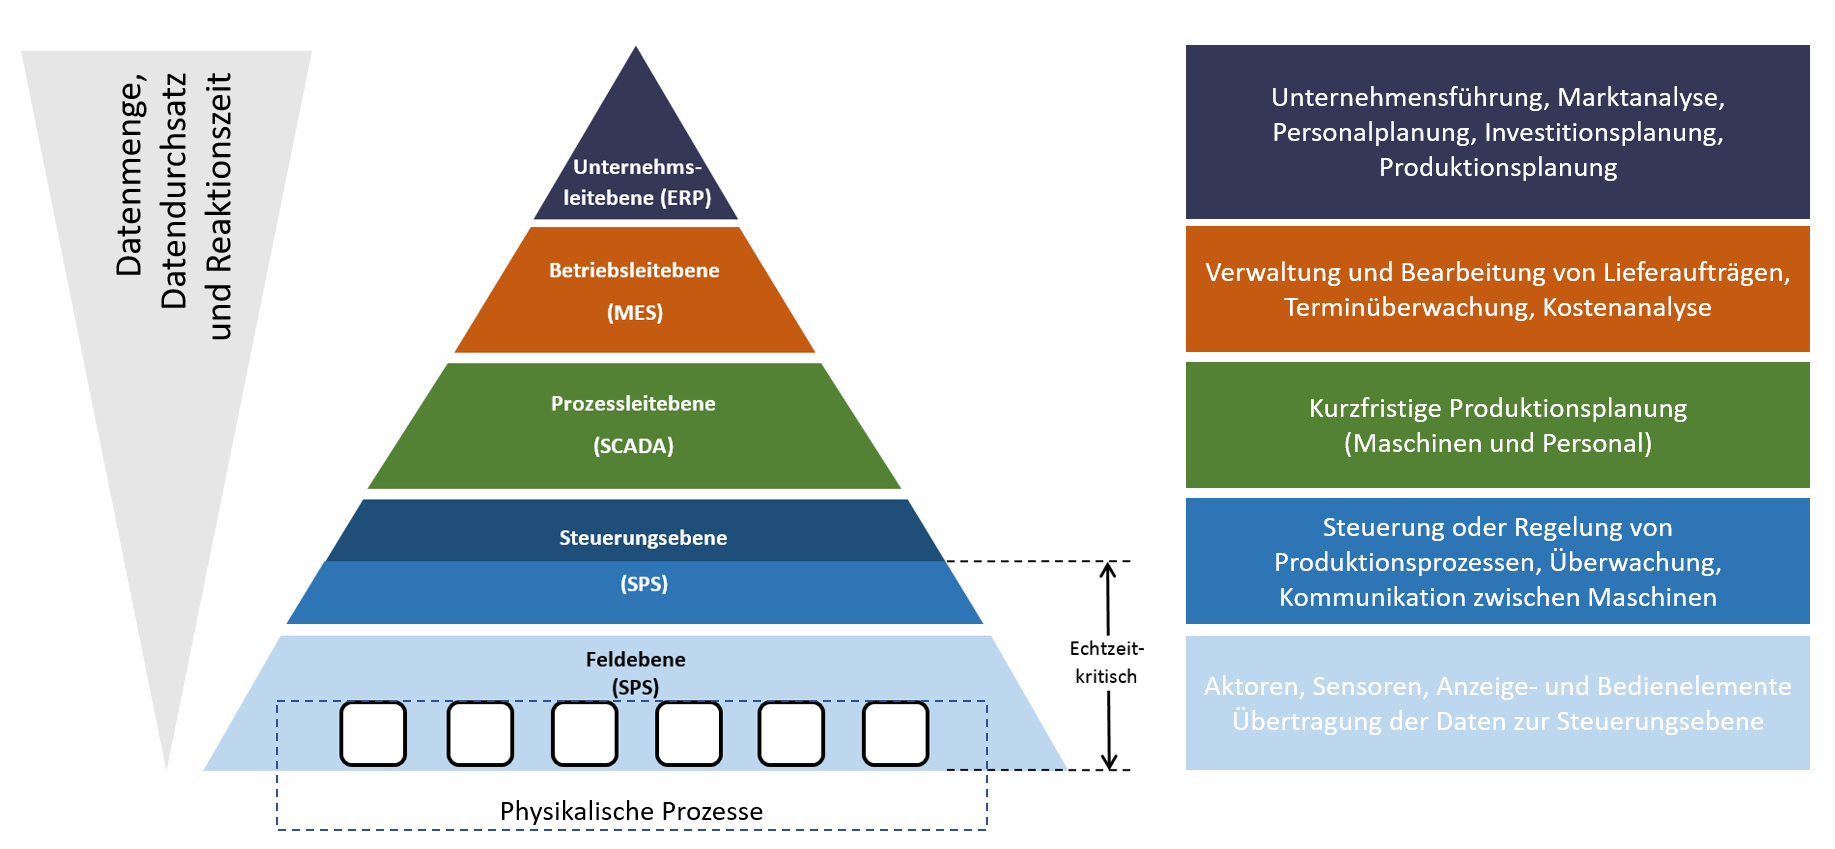
\includegraphics[width=0.9\textwidth]{images/Automatisierungspyramide.png}
		\caption{Automatisierungspyramide.}
		\label{fig:Automatisierungspyramide}
	\end{center}	
\end{figure}

In den folgenden Kapitel werden die Definitionen einiger Grundbegriffe der Automatisierungstechnik erläutert. Daraus werden die Ziele der Automatisierungstechnik abgeleitet und Kategorisierungen der Prozesse beschrieben. Es folgt ein kurzer Ausblick auf die zusätzliche Hardware, um IT-Systeme zu OT fähigen Systemen zu erweitern. Abgeschlossen wird diese Kapitel mit der Funktionsbeschreibung von Speicherprogrammierbaren Steuerungen.  


\subsection{Grundlagen zur Automatisierung}

\subsubsection{Begriffsdefinitionen}

Die Automatisierungstechnik ist das technische Fachgebiet, das sich mit Technologien und Methoden beschäftigt, um einzelne Arbeitsschritte, zusammenhängende Arbeitsschritte oder den gesamten Umfang von Arbeitsschritten eines Prozesses mit Hilfe von Anlagen, Maschinen und Geräten ohne menschliches Zutun auszuführen.

Ein Prozess wird nach \cite{AmericanNationalStandards.} als eine Reihe miteinander verbundener Aufgaben, die gemeinsam Inputs in Outputs umwandeln definiert, siehe Abbildung \ref{fig:Prozess}. 


\begin{figure}[H]
	\begin{center}
		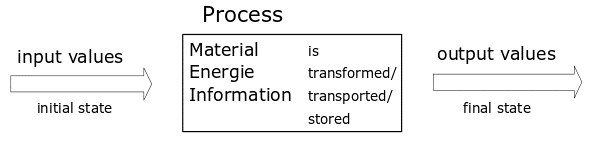
\includegraphics[width=0.6\textwidth]{images/Prozess.png}
		\caption[Prozesse in der Automatisierungstechnik.]{Darstellung eines Prozesses im Sinne der Automatisierungstechnik mit Eingangsgrößen, transformation durch Material, Energie und Informationseinbringung und Ausgangsgrößen als Ergebnis des Prozesses. \cite{Heimbold.2015}}
		\label{fig:Prozess}
	\end{center}	
\end{figure}

Damit der Prozess technisch umsetzbar ist, bedarf es einem System (Anlage, Maschine oder Gerät) welches mit Hilfe der Prozessleittechnik entwickelt wird. Die Prozessleittechnik ist die Ingenieursdisziplin, welche sich mit den Architekturen, Mechanismen und Algorithmen zur Aufrechterhaltung des Outputs eines bestimmten Prozesses, innerhalb eines gewünschten Bereichs befasst. Das wechselseitige Verhalten zwischen Prozess und technischem System ist in Abbildung \ref{fig:ProzessUndSystem} dargestellt.

\begin{figure}[H]
	\begin{center}
		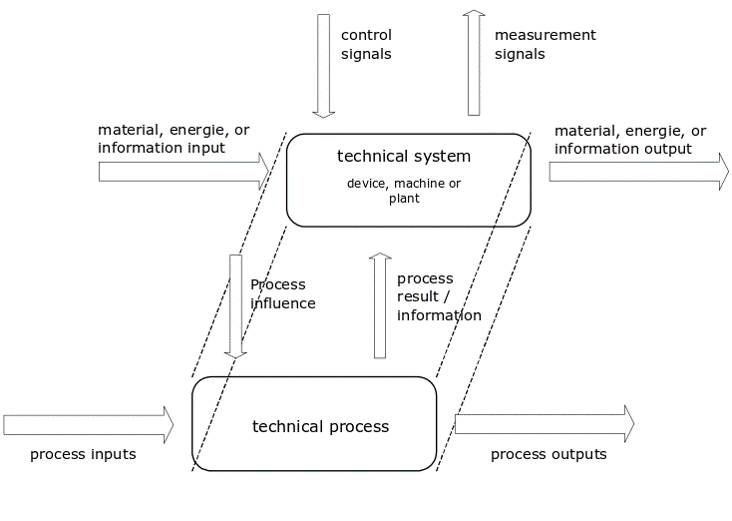
\includegraphics[width=0.6\textwidth]{images/ProzessIneinemTechnischenSystem.png}
		\caption{Darstellung eines Prozesses welcher durch ein technisches System ermöglicht wird. \cite{Heimbold.2015}}
		\label{fig:ProzessUndSystem}
	\end{center}	
\end{figure}


Das technische System übernimmt dabei die Grundfunktionalitäten für Steuerungs-, Regelungs-, und Visualisierungs-Vorgägne. Diese Funktionen werden allgemein mit dem Begriff Automatisierung zusammengefasst. Dabei übernimmt eine Steuerung - für welche sich Speicherprogrammierbare Steuerungen (SPS) und Industrie-PC's (IPC) als Standard etabliert haben - die Aufgaben Entscheidungen für Arbeitsschritte zu treffen bzw. Prozessgrößen zu regel. Die Basis, zur Umsetzung dieser Aufgaben, ist ein vorgefertigtes Programm, welches vorgegebene Führungsgrößen und rückgeführte Prozessgrößen aus der Anlage sowie Daten aus internen Speichern des Systems verwendet und durch logische und mathematische zusammenhänge neue Stellgrößen bestimmt. \cite{Wellenreuther.2015}

Hier ist eine Unterscheidung der Grundfunktionen von steuern und regeln angebracht. Steuern bedeutet, dass das System Ausgangsgrößen bestimmt, auf Grund von vordefinierten Systemverhalten. Die Zielgrößen werden dabei nicht erfasst und Störeinflüsse sind nicht kompensierbar. Häufig werden Steuerungen mit digitalen Messgrößen, wie z.B. Näherungsschaltern versehen, um weitere Prozessschritte einzuleiten. Diese Art des Steuerns wird als Ablaufsteuerung bezeichnet, sie sind die am meisten implementierten Steuerungen in der Praxis. \\
Beim Regeln wird, durch kontinuierliche Messungen der Prozessparameter die Abweichung zu den Vorgabeparametern verglichen. Der dabei entstehende Fehler wird durch einen Regler, der die Stellgröße im System vorgibt, versucht auszugleichen. Störeinflüsse können somit kompensiert werden. Bei komplexen Automatisierungssystemen werden prozessschrittspezifische Vorgabeparameter benötigt. Diese werden in der Regel durch eine Ablaufsteuerungen an die Regler übergeben.      


\subsubsection{Ziele der Automatisierung}

Mit einer Automation von Prozessen bzw. Produktionsanlagen werden unterschiedliche Ziele verfolgt. Teilweise können diese Ziele im Widerspruch stehen, sodass eine Priorisierung auf anlagen- und unternehmensspezifische Eigenschaften erfolgen muss. Nach \cite{Heimbold.2015} können vier Kernziele Formuliert werden, 

\begin{itemize}
	\item Steigerung der Qualität,
	\item Humanisierung,
	\item Steigerung der Sicherheit und
	\item Rationalisierung.
\end{itemize}

Maschinen und Anlagen können in vielen Bereichen effizienter und mit gleichbleibender Genauigkeit arbeiten. In einem vollautomatisierten Produktionssystem werden jedoch viele Fehler nicht direkt erkannt. Darum sind explizite Qualitätssicherungssysteme notwendig um die grundsätzlich hohe maschinelle Qualität für alle produzierten Teile garantieren zu können. Diese zusätzlichen Arbeitsschritte erfordern eine Erhöhung der Durchlaufzeiten und erzeugen erhöhte Komplexität, was zu einem Widerspruch zwischen Qualität und Rationalität führt. 

Für den Menschen unangenehme oder sogar gefährliche Arbeiten können durch den Einsatz automatisierter Systeme übernommen werden. Dabei spielt die Varianz der Tätigkeiten eine große Rolle wie das Automationssystem aufgebaut werden muss. Da bei hoher Varianz der Arbeitsschritte eine komplexe Anlage benötigt wird, ist es häufig der Fall, dass diese Anlagen keinen wirtschaftlichen Vorteil bringen und somit nicht realisiert werden.

In anderen Produktionsprozessen kommt es vor, dass Mensch und Maschinen eng zusammenarbeiten müssen. Dadurch ist das Entwickeln von sicheren Maschinen in den Bereichen, wo Mensch und Maschine Hand in Hand arbeiten müssen, ein großes Forschungsfeld. Die möglichen Sicherheitskonzepte und sicherheitstechnischen Komponenten sind vielfältig und erfordern kreative Lösungsansätze. Erschwerend ist hier die Notwendigkeit, die heutzutage gültigen, Normen,  Maschinen- und Arbeitsplatzrichtlinien einzuhalten.

   

\subsubsection{Klassifizierung von Prozessen}

Durch die Einteilung der Prozesse in verschiedene Klassen, lassen sich direkt unterschiedliche Anforderungen auf das Automatisierungssystem ableiten. Eine Klassifizierung von Prozessen ist anhand verschiedener Kriterien, wie Art des Medium, Art der Einwirkung, Art der stofflichen Umwandlung bzw. Transports, Art der Prozessgrößen und dem zeitlichen Ablauf, möglich. Diese Einteilungen, siehe Abbildung \ref{fig:Klassifizierung}, ermöglichen es im Vorfeld auswählen zu können, welche Entwicklungsverfahren und Methoden  - auch das notwendige Fachwissen - geeignet sind, um eine Automatisierung umzusetzen. 

\begin{figure}[H]
	\begin{center}
		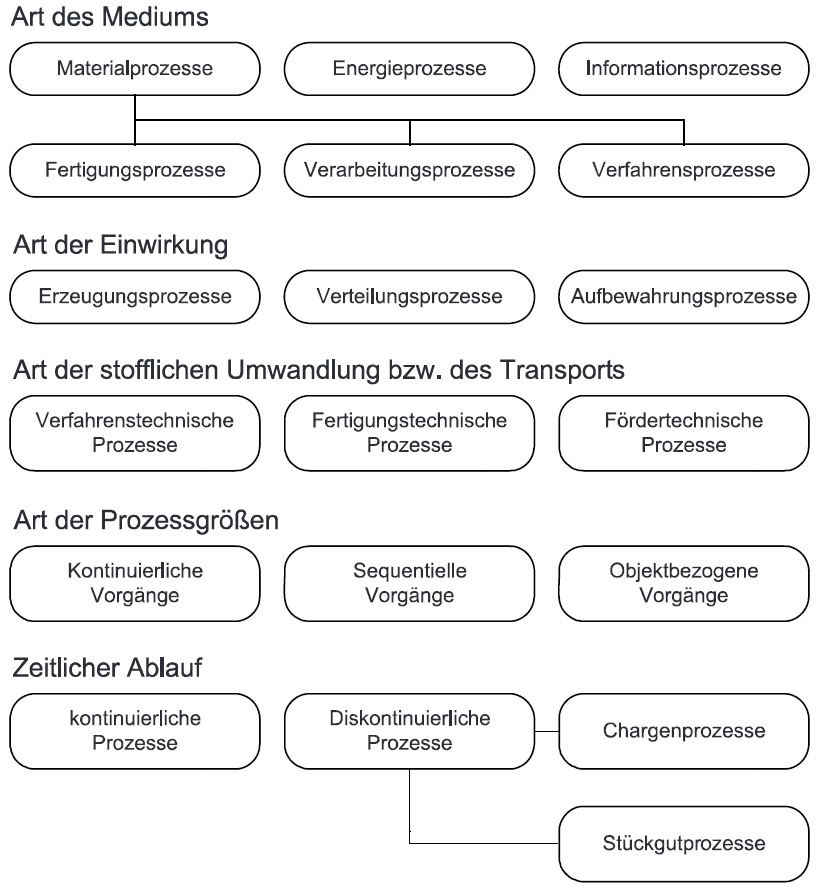
\includegraphics[width=0.6\textwidth]{images/Klassifizierung.png}
		\caption[Klassifizierung von Prozessen der Automatisierungstechnik.]{Klassifizierung der Prozesse nach Art des Mediums, Art der Einwirkung, Art der stofflichen Umwandlung, Art der Prozessgrößen und dem zeitlichen Ablauf. \cite{Heimbold.2015}}
		\label{fig:Klassifizierung}
	\end{center}	
\end{figure}

So wird eine Fertigung von Getrieben klassifiziert durch die Medienart als Materialprozess mit Einwirkungen durch Erzeugungs-, Verteilungs- und Aufbewahrungsprozessschritten in Sequentiellen Vorgängen und diskontinuierlichen Zeitabläufen. Diese Art von Prozessen ist für die weiteren Inhalte der Lehrveranstaltung relevant.  

Eine anderes Beispiel für eine Klassifizierung nach diesem Modell ist der Erzeugungsprozess von Medikamenten, welcher ein verfahrenstechnischer Materialerzeugungsprozess mit kontinuierlichen und sequentiellen Vorgängen ist.   



\subsection{Speicherprogrammierbare Steuerung - SPS}

Derzeit sind Speicherprogrammierbare Steuerungen die am meisten verbreitete Hardware für Automatisierung von Maschinen und Anlagen. Mittlerweile haben sich hier zwei Varianten etabliert. Zum einen eine Hard-SPS mit speziell entwickelter Hardware. Diese besteht aus einer Stromversorgung, einem Steuerungsprozessor CPU, zentralen digitalen Eingangs- und Ausgangsbaugruppen sowie einem internen Bussystem. Andererseits haben sich vor allem in den vergangen Jahren Soft-SPS  im Markt etabliert. Diese besitzen Standardkomponenten aus PC-Systemen und verfügen über ein herkömmliches Betriebssystem (z.B. Windows). Somit wird ermöglicht, dass andere Software, wie z.B. C++ Programme, auf dem Industrie-PC ausgeführt werden kann.\\
Damit sich die rechnerinternen Prozesse nicht gegenseitig blockieren, bedarf es spezieller Softwarearchitektur, die es ermöglicht, den SPS-Code echtzeitfähig abzuarbeiten. Der Teil, der dies ermöglicht, wird als Laufzeit (eng. Runtime) bezeichnet und ersetzt die speziell entwickelte Hardware CPU der Hard-SPS. Als Kommunikationsschnittstelle zu den Busklemmen dient ein Feldbussystem (EtherCAT, ProfiNet, o.ä.). Moderne standard Netzwerkkarten können so konfiguriert werden, dass sie zum Master des Feldbussystems werden. Beide SPS-Varianten unterliegen der SPS-Norm, welche im folgenden Kapitel besprochen wird.  

\subsubsection{SPS-Norm DIN EN 61131-3 (IEC 61131-3)}

Die Programmierung von automatisierten Systemen ist in der Regel sehr anwendungsspezifisch, jedoch soll durch die SPS-Norm ein rationelleres und herstellerunabhängiges Programmerstellungskonzept entstehen. Zu diesem Zweck führt die Norm vier Grundkonzepte ein, welche dabei helfen sollen möglichst allgemeine und wiederverwendbare Programmbausteine zu entwickeln. In diese Bausteinen sind Anwendungsspezifische SPS-Operanden, Eingänge, Ausgänge, Zählern und Zeitglieder sowie Merkern nicht einzusetzen. Erst bei der Erstellung des übergeordneten Anlagenprogramms sollen anlagenspezifische Zuweisungen, Zähler und Merker an die Bausteine übergeben bzw. in der Ablaufsteuerung berücksichtigt werden. Die vier Konzepte sind in nachfolgenden Punkten näher beschrieben.  

\begin{itemize}
	
\item[1.] \textbf{Datentypen}

Eine einheitliche Definition für Datentypen, Konstanten und Variable sind verbindlich vorgeschrieben. Für symbolische und absolute Adressierungen sind die definierten Datentypen Grundlage der expliziten Ausführung der Variablendeklaration. \cite{Wellenreuther.2015} 
Eine Auflistung der wichtigsten Datentypen ist in Tabelle \ref{tab:Datentypen} zu sehen. 



\item[2.] \textbf{Programmorganisationseinheiten (POU's)}

Programmorganisationseinheiten sind hierarchisch gegliederte Programmeinheiten, welche aus einem Hauptprogrammtypen (\textit{Program}) mit Zugriff auf E/A-Operanden und zwei Unterprogrammtypen mit und ohne Speichermöglichkeit (mit \textit{Function\_Block} und ohne \textit{Function}) besteht. \cite{Wellenreuther.2015} In Abbildung \ref{fig:Programmorganisationseinheit} ist der hierarchische Aufbau  und die Aufrufmöglichkeiten dargestellt.  
Aus dieser Organisationsform heraus, lassen sich verallgemeinerte Programmbausteine erstellen, welche beliebig oft in einer oder mehreren Anlagen eingesetzt werden können. Dadurch wird sichergestellt, dass bei immer wachsendem Automatisierungsaufwand von komplexer werdenden Anlagen, die Steuerungsentwicklung nicht im gleichen Maße ansteigt. Aus den entwickelten Bausteinen können dafür auch Bibliotheken angelegt werden.

\begin{figure}[H]
	\begin{center}
		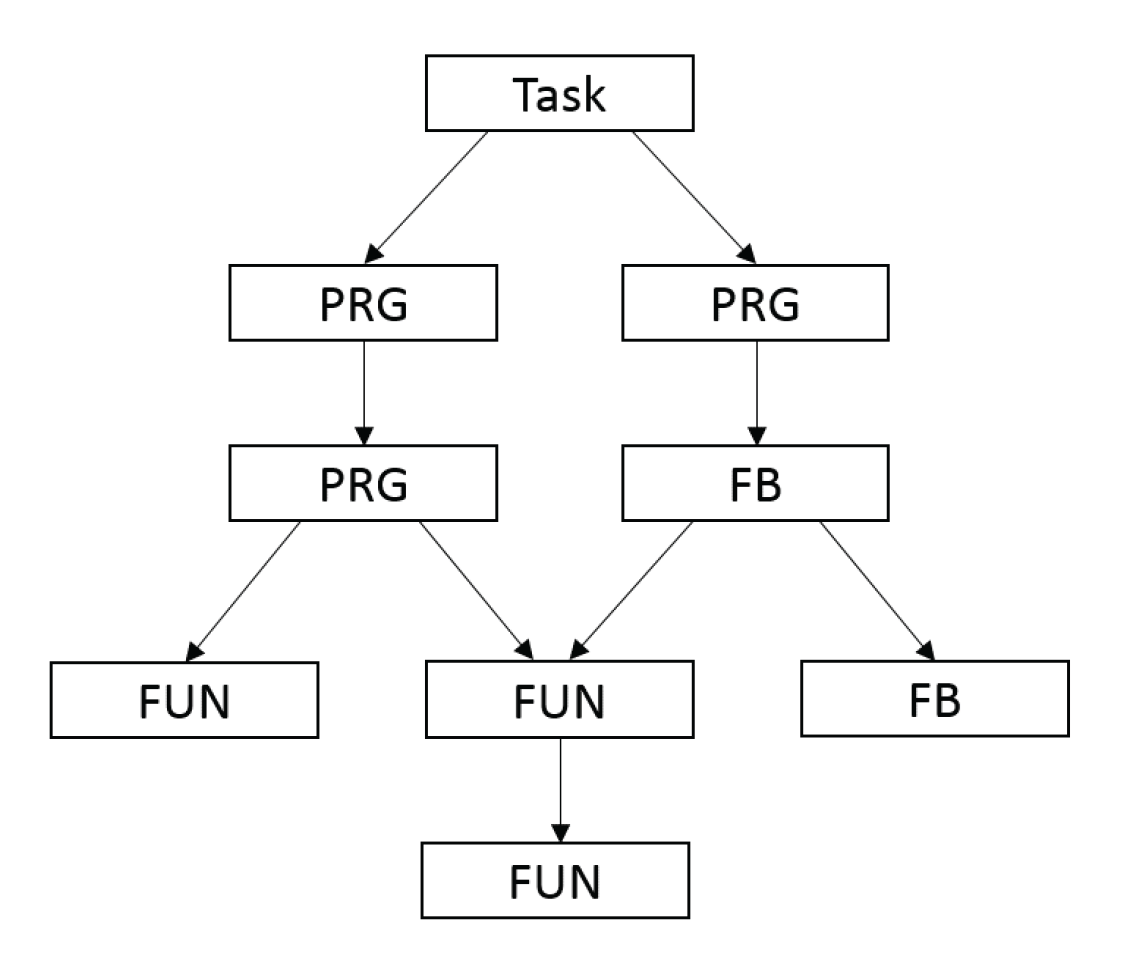
\includegraphics[width=0.45\textwidth]{images/POUs.png}
		\caption{Struktur der POU's innerhalb eines Task.}
		\label{fig:Programmorganisationseinheit}
	\end{center}	
\end{figure}

\item[3.] \textbf{Programmiersprachen}

Um die Varianz der Anwendungsfälle und der Programmierkenntnisse der Steuerungsentwickler abzudecken sind fünf Programmiersprachen zur Programmentwicklung zur Verfügung gestellt. Diese ermöglichen eine grafische bzw. textuelle Programmerstellung und können z.B. Relaissteuerungen mittels dem Kontaktplan (KOP) oder Abläufe durch die Ablaufsprache (AS) einfach realisieren. Eine weitere grafische Programmsprache liegt mit der Funktionsbausteinsprache (FBS/FUP) vor. Textuelle Programmiersprachen sind die Anweisungsliste (AWL), für die Programmierung von lineare Prozesse, oder der Sturkturierte Text (ST), mit hochsprachenähnlichen Funktionalitäten. Während dieser Lehrveranstalltung wird ausschließlich mit ST gearbeitet. Beispiele von weiteren Programmiermöglichkeiten sind im Anhang \ref{} dokumentiert. 

Einige SPS-Systeme bieten auch die Möglichkeit UML-Graphen zur erstellen. Dabei kann ein Zustandsgraphen, siehe Kapitel \ref{sec:Zustandsgraphen}, direkt erstellt und bei Programmausführung verwendet. \cite{Fowler.2004}

\item[4.] \textbf{Programmablauf}

Der Programmablauf basiert auf dem Taskkonzept, welches die Ausführung der Programmorganisationseinheiten priorisiert und zeitzyklisch oder ereignisorientiert abarbeitet. Bei der Entwicklung des Steuerungsprogramms muss der Code nach den zeitzyklischen oder ereignisorientierten Anforderungen entworfen werden. Die zyklische Abarbeitung eines Tasks ist in Abbildung \ref{fig:Programmablauf} dargestellt.

\begin{figure}[H]
	\begin{center}
		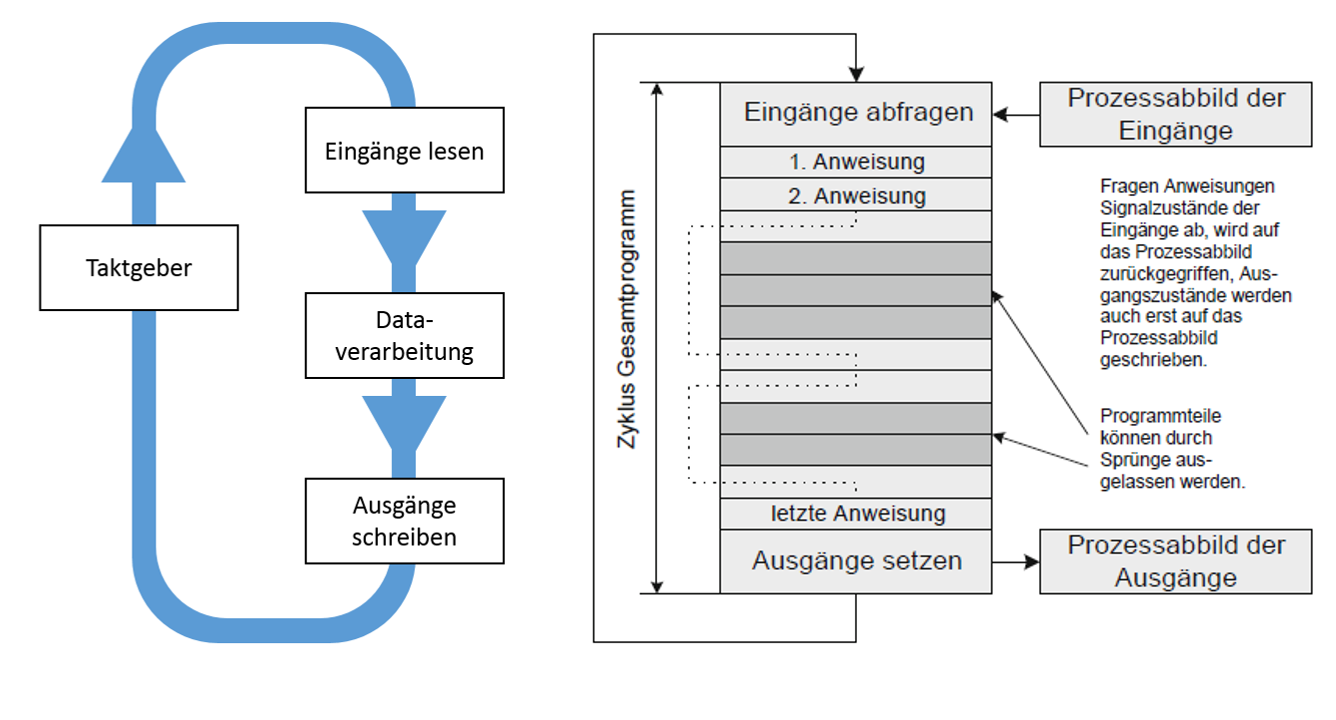
\includegraphics[width=0.8\textwidth]{images/Programmablauf.png}
		\caption{Ablauf eines Tasks durch zyklische Abarbeitung.}
		\label{fig:Programmablauf}
	\end{center}	
\end{figure}

\end{itemize}


Zusätzlich sind zwei weitere Funktionalitäten in der Beckhoff TwinCAT SPS implementiert, diese sind auch in Systemen anderer Hersteller vorhanden, die Anwenderspezifische Datentypen und Globale Variablen Listen. 

\begin{itemize}
	\item[5.] \textbf{Data Unit Type (DUT)- Anwenderspezifische Datentypen}
	
	Zusätzlich zu den Standard-Datentypen können Sie eigene Datentypen wie Strukturen, Aufzählungen/Enumeration, Referenzen und Unions definieren. Diese legen Sie als DUT an \cite{InfosysDUT}.
	
	\item[6.] \textbf{Globale Variablen Listen (GVL)}
	
	Der Inhalt von Globalen Variablen Listen ist innerhalb des SPS-Projektes für alle POU's zugreifbar \cite{InfosysGVL}. Deswegen eignen sie sich für die Verwendung von Hardware oder HMI Schnittstellen. 
\end{itemize}


\subsubsection{E/A-Geräte}

Alle Prozesssignale müssen durch E/A-Geräte erfasst bzw. gesetzt werden. Damit der Verkabelungsaufwand geringer wird, kommunizieren die E/A-Geräte mit der SPS (CPU) über Feldbussysteme. Dieses Konzept ist bei Soft-SPS immer notwendig, Hard-SPS kann in vielen Fällen,  durch direkten Anschluss der Klemmen an die SPS, auf das Feldbussystem verzichten. Der Feldbus wird durch Buskoppler auf einen lokalen Klemmenbus übersetzt und galvanisch getrennt. Die Eingangsgeräte schreiben ihre Werte aus den Prozesssignalen auf den Klemmenbus, während die Ausgangsgeräte die Klemmenbussignale lesen und die Prozesssignale setzen. Die Prozesssignale und der Klemmenbus sind ebenfalls galvanisch getrennt, wodurch bei Störungen die Bussysteme nicht beeinträchtigt werden. Abbildung \ref{fig:SPS-Hardware} stellt den Aufbau einer SPS mit Klemmen und den dazugehörigen Bussystemen dar. 

\begin{figure}[H]
	\begin{center}
		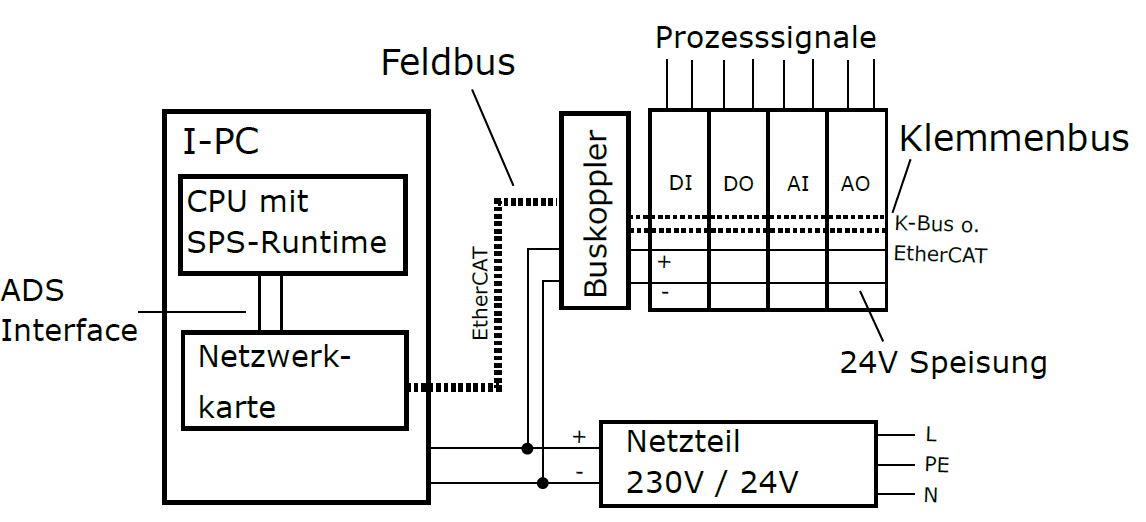
\includegraphics[width=0.9\textwidth]{images/SPS_Hardware.png}
		\caption[Darstellung der SPS-Hardware.]{Darstellung der SPS-Hardware für einen I-PC mit Soft-SPS Laufzeit. Angelehnt an das Beckhoff SPS-System.}
		\label{fig:SPS-Hardware}
	\end{center}	
\end{figure}

\textbf{Adressierung von Prozesssignalen}

Angesprochen werden die Prozesssignale durch Adressen. Diese sind flexibel oder explizit zu vergeben. Mit \textrm{AT\%I*} oder \textrm{AT\%Q*} können flexible Adressbits vergeben werden.  Die Größe der zu übertragenden Datenbits werden bei dieser Art automatisch festgestellt. Die endgültige Zuweisung auf einen Klemmenkanal erfolgt durch manuelle Verknüpfung. Zusätzlich zu den Ein- Ausgangsspeicherpräfix I und Q gibt es noch einen Merkerspeicherbereich, welcher mit dem Präfix M adressiert werden kann. 

Die explizite Adressierung von Ein- und Ausgangsvaribalen ist in Tabelle \ref{tab:Adressierung} aufgelistet.

 



\subsubsection{Digitale Ein- / Ausgangsklemmen}

Digitale Signale, auch als binäre Signale bezeichnet, haben eine Wertezuweisungen von logischer 0 oder 1 in der Steuerung. Da es sich jedoch um reale Signale aus dem Prozess handelt, muss definiert sein, welches Spannungsniveau die logische 0 und 1 darstellt. Gängige Spannungen sind \SI{3}{\volt}, \SI{4}{\volt}, \SI{12}{\volt} oder \SI{24}{\volt}, wobei es hier nicht um die Schaltniveaus handelt, sonder um die Nennspannung. Da reale Signale niemals den genauen Spannungswert annehmen. Auf Grund von Störungen und Leitungswiderständen werden Schaltniveaus festgelegt, welche sich in einer Hysteresiskurve darstellen lassen, siehe Abbildung \ref{fig:Hysteresis}. 

\begin{figure}[H]
	\begin{center}
		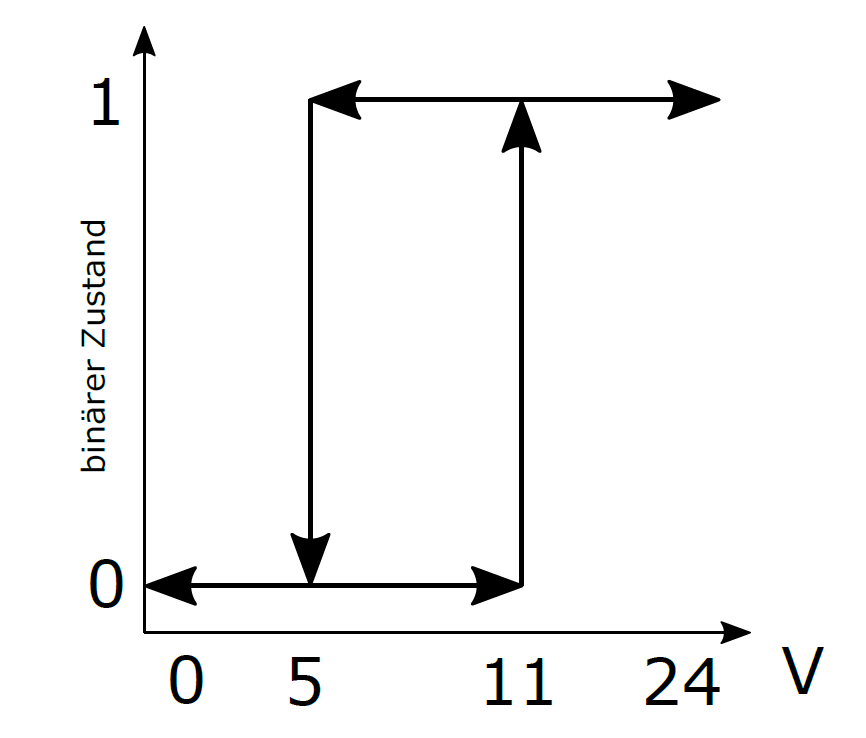
\includegraphics[width=0.4\textwidth]{images/Hysteresis.png}
		\caption{Hysteresiskurve von einem digitalen Eingang mit 24V Nennspannung.}
		\label{fig:Hysteresis}
	\end{center}	
\end{figure}

\textbf{Digitale Eingangsklemmen}

Bei der Auswahl von digitalen E/A-Klemmen ist es entscheidend die Art des Sensors zu berücksichtigen. Dabei gibt es eine grundlegende Unterscheidung zwischen 2-Leiter- und 3-Leiter-Sensoren. Das Schaltbild mit Busklemme ist in Abbildung \ref{fig:SchaltbildDigitaleSensoren} für beide Ausführungen zu sehen. 3-Leiter-Sensoren benötigen im nicht ausgelösten Zustand weniger Leistung als 2-Leiter-Sensoren, da kein Reststrom für die Leistungsversorgung erforderlich ist.

Ein weiterer wichtiger Faktor ist die Bestimmung, ob der Sensor als Stromquelle oder als Stromsenke ausgeführt ist. Sensoren, die als Stromquelle agieren, werden als PNP (Positive-Negative-Positive) bezeichnet. In diesem Fall muss das Eingangsgerät als Stromsenke fungieren. Digitale Eingangsgeräte mit einer Senkenfunktion sind beispielsweise die Modelle EL100x \& EL101x. Falls der Sensor jedoch als NPN (Negative-Positive-Negative) Sensor konfiguriert ist, ändert sich die Richtung des Stromflusses. In diesem Fall sollte ein passendes Eingangsgerät mit Quellfunktionalität am Eingang ausgewählt werden, wie beispielsweise die Modelle EL108x \& EL109x.

\begin{figure}[H]
	\begin{center}
		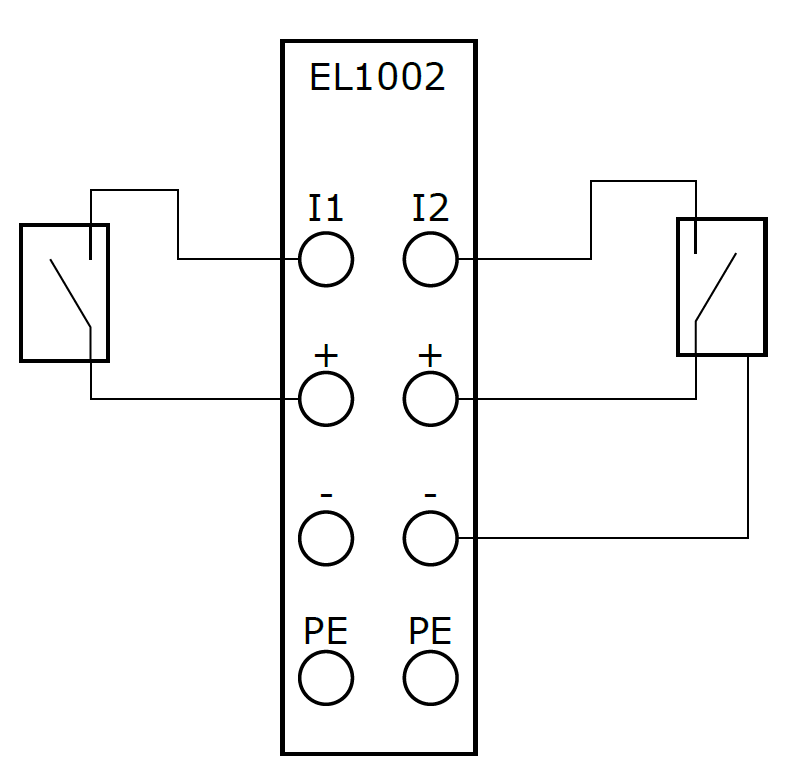
\includegraphics[width=0.4\textwidth]{images/SchaltbildDigitaleSensoren.png}
		\caption[Schaltbild für digitale Sensor Anschlüsse.]{Schaltbild für 2-Leiter Sensor (links am Eingang I1) und 3-Leiter Sensor (rechts am Eingang I2) mit Busklemme EL1002 für PNP-Schaltung. [Abgeleitet aus dem Beckhoff-Infosys]}
		\label{fig:SchaltbildDigitaleSensoren}
	\end{center}	
\end{figure}


Die Schaltzustände der Sensoren werden häufig mit "normaly open" (NO) und "normaly closed" (NC) bezeichnet. Dies bezieht sich auf das Verhalten der Sensoren im nicht aktiven Zustand. Hier steht bei NO kein Signal am Eingangsgerät an und innerhalb der SPS der Wert 0 (\textrm{FLASE}) angezeigt. Bei NC steht ein Signal an und der Wert 1 (\textrm{TRUE}) wird angezeigt. Die Schaltsymbole für NO und NC werden in Abbildung \ref{fig:Schaltzustaende} dargestellt.

\begin{figure}[H]
	\begin{center}
		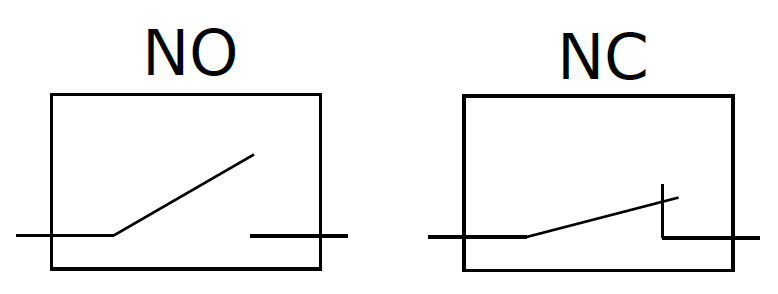
\includegraphics[width=0.4\textwidth]{images/Schaltzustände.png}
		\caption{Schaltsymbole für Sensoren mit NO und NC Verhalten.}
		\label{fig:Schaltzustaende}
	\end{center}	
\end{figure}

 
Mechanische Taster neigen aufgrund des Prellens, also des wiederholten Öffnens und Schließens des Kontakts, aufgrund elastischer Materialverformungen, dazu, keine eindeutig definierte Flanke zu erzeugen. Dieses Verhalten kann zu Fehlern im Steuerungsprogramm führen. Jedoch kann das Signal durch Eingangsfilter mit längeren Schaltzeiten, beispielsweise \SI{3}{\milli\second}, geglättet werden. Auf diese Weise wird sichergestellt, dass beim Wechsel der Schalterstellung eine klare Flanke erzeugt wird, siehe Abbildung \ref{fig:Prellfilter}.

\begin{figure}[H]
	\begin{center}
		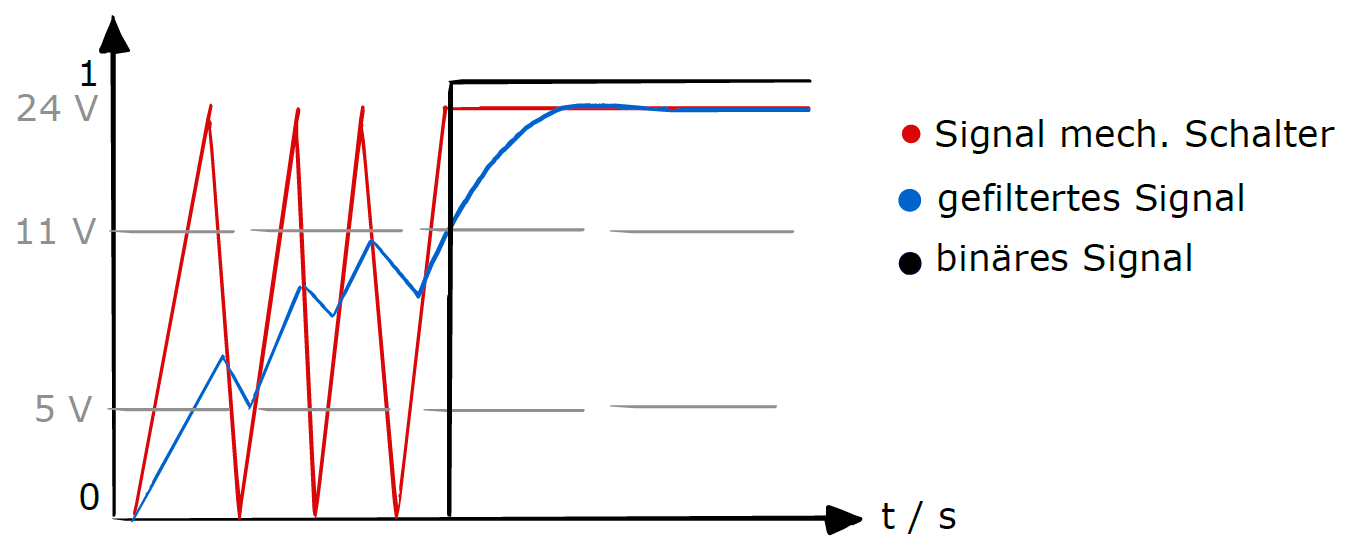
\includegraphics[width=0.7\textwidth]{images/Prellfilter.png}
		\caption{Eingangsgefiltertes Signal zum Schutz vor Prellung.}
		\label{fig:Prellfilter}
	\end{center}	
\end{figure}

\textbf{Digitale Ausgangsklemmen}

Digitale Ausgangsklemmen bei SPS dienen dazu, digitale Signale (bzw. binäre Signale) an externe Geräte oder Aktoren zu senden. Sie können dazu verwendet werden, elektrische Signale zu schalten und somit Prozesse in der realen Welt zu steuern. Das Schalten der Signale kann durch Relais aber auch Halbleiterschalter realisiert werden. Weiters kann es eine interne (Typ 2) oder externe (Typ 1) Spannungsversorgung geben, siehe Abbildung \ref{fig:DOTypen}. Bei externer Versorgung können teilweise größere Leistungen geschalten werden. Binärausgänge schalten oft induktive Lasten. Dies kann beim Trennen des Stromkreises zu hohen Spannungsspitzen führen. Eine Freilaufdiode verhindert das auftreten dieser Spitzen. \cite{Becker.2014}

Die Standartklemmen für digitale Ausgänge (DO) sind mit unterschiedlichen Nennstrom erhältlich. So hat haben die Klemmenmodelle EL200x, zwei, vier oder acht Kanäle mit $\SI{24}{\volt}_{DC}$ mit \SI{0,5}{\A} und die Modelle EL202x, zwei oder vier Kanäle mit $\SI{24}{\volt}_{DC}$ bei \SI{2}{\A}. Weitere Klemmen mit zusätzlichen Diagnosefunktionen, wie Drahtbrucherkennung, sind ebenfalls erhältlich. \\
Weiters können DO auch nach dem Prinzip PNP und NPN arbeiten. So kann bei externen Spannungsversorgung die Masse (\SI{0}{\volt}) als Ausgang durchgeschalten werden, wie bei der Klemme EL208x. \\
Neben den klassischen DO's gibt es noch  weiter Ausführungsvarianten, von Push-Pull-Qutputs mit Tristate, Pulsweiten modulierte (PWM) Ausgänge für Aktoren bzw. zur LED-Steuerung oder, für spezielle Anwendungsfälle, PWM Lichtwellenleiter Ausgangssignal. \cite{InfosysEL2xxx}


\begin{figure}[H]
	\begin{center}
		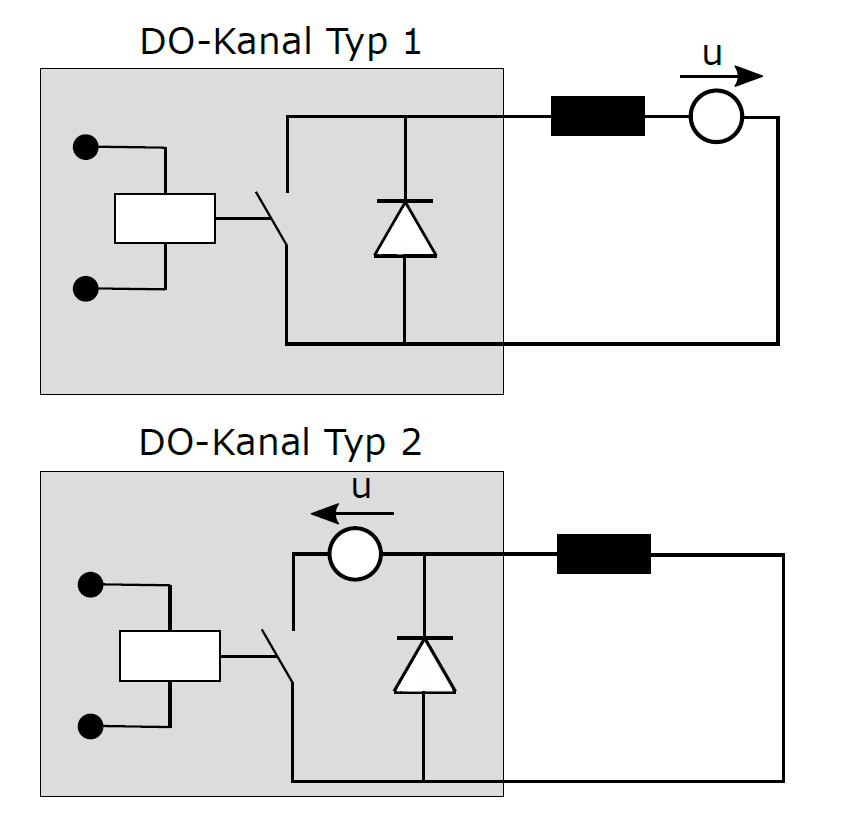
\includegraphics[width=0.4\textwidth]{images/DOTypen.png}
		\caption{Schaltbilder von digitalen Ausgängen mit interner und externer Spannungsversorgung.\cite{Becker.2014}}
		\label{fig:DOTypen}
	\end{center}	
\end{figure}



\subsubsection{TwinCAT Einführung}

Eine vollständige Einführung in TwinCAT wird hier nicht besprochen. Die folgenden Abschnitte dienen dazu einen allgemeinen Überblick über die TwinCAT Entwicklungsumgebung zu bekommen. Die vollständige Dokumentation der Benutzeroberfläche und der TwinCAT-Projekt Struktur finden Sie im Beckhoff-Infosys unter \cite{InfosysBenutzeroberflaeche} und \cite{InfosysTwinCATProjekte}. Erste Schritte in der TwinCAT 3 Entwicklungsumgebung werden in der Vorlesung besprochen und es können Tutorial Videos wie \url{https://www.youtube.com/watch?v=GOFUsWc61Hk&t=21s} von Christian Stöcker angesehen werden.
 
\textbf{Projekterstellung und Lizenzierung}

Die Entwicklungsumgebung TwinCAT 3 ist in Visual Studio eingebettet, entweder in ein vorinstalliertes Visual Studio oder, wenn noch keines vorhanden ist, in eine Visual Studio Shell, die bei der TwinCAT 3 installation automatisch mit installiert wird. Für jede Automatisierungsaufgabe wird in einem eigenen Projekt gearbeitet. Der Ordner in dem das Projekt gespeichert wird kann vorzugsweise den gleichen Namen wie das Projektes besitzen. Standardmäßig speichert TwinCAT alle Projekte in den Pfad (C:\textbackslash\,Users\textbackslash\,[your user]\textbackslash\,Documents\textbackslash\,TcXaeShell). Da innerhalb der Entwicklungsumgebung auf Bibliothekspfade referenziert wird und diese nicht auf allen PC's identisch sind, gibt es ein Austauschformat .tnzip. Dieses kann unter \textrm{Datei/Save Project as Archive} gespeichert werden und durch \textrm{Datei/Öffnen/Open Solution from Archive} geöffnet werden. Beim Öffnen muss das extrahierte Projekt lokal in einen neuen Ordner gespeichert werden. 

Des weiteren muss eine Soft-SPS Instanz angelegt werden. Innerhalb eines Projektes können auch mehrere SPS-Projekte entwickelt und auf einem IPC ausgeführt werden. Für solche SPS Instanzen sind vorgefertigte Templates zur Verfügung, welche eine standardisierte Projektstruktur nach der IEC 61131-3 beinhalten. Die Erstellung erfolgt durch Rechtsklick auf den SPS Baustein am linken Bildrand mit \textrm{Neues Element hinzufügen/Standard PLC Project}. Namensgebung der SPS-Instance ist zum Beispiel SPS oder bei mehreren Instanzen SPS1 und SPS2.\\
Eine Taskreferenz zum Programm \textrm{Main} ist bereits angelegt und mit einer Zykluszeit von \SI{10}{\milli\second} im System hinterlegt. 

Eine erstmalige Programmausführung ist ab diesem Zeitpunkt möglich - auch wenn noch kein Code vorhanden ist. Dazu muss das Projekt durch die Schaltfläche \textrm{Konfiguration aktivieren} 
\includegraphics[height=10pt]{images/IconKA.png}  in die Laufzeit geladen werden. Im Anschluss kann das Zielsystem (die Soft-SPS) in den \textrm{Run Mode} 
\includegraphics[height=10pt]{images/Runmode.png} versetzt werden. Dafür werden Lizenzen abgefraget, diese können durch Eingabe eines Codes für Entwickler immer für sieben Tage freigegeben werden, siehe Abbildung \ref{fig:Lizenzschluessel}.   

\begin{figure}[H]
	\begin{center}
		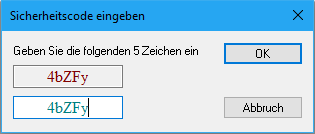
\includegraphics[width=0.4\textwidth]{images/Lizenzschluessel.png}
		\caption[Lizenzaktivierung TwinCAT 3.]{Eingabe des Lizenzschlüssel zur Aktivierung der Lizenzen für sieben Tage. Beliebig oft wiederholbar.}
		\label{fig:Lizenzschluessel}
	\end{center}	
\end{figure}
				

\textbf{Konfig- und Runmodus}

Der oben genannte \textrm{Run Mode} ist einer von drei Modi, die die Laufzeit (Runtime) der SPS annehmen kann, die Symbole sind in Abbildung \ref{fig:Laufzeitmodi} dargestellt. Grundsätzlich ist beim Entwickeln die Laufzeit im \textrm{Konfig Mode}. Wie der Name schon vermuten lässt, kann in diesem Modus die SPS konfiguriert werden. D.h. die Zykluszeiten und Priorisierung der Tasks kann eingestellt werde, neue Programme und Programmsegmente können erzeugt werden u.v.m.. 

Der zweite Modus ist der \textrm{Free Run Mode}. Mit diesem ist es möglich Peripheriegeräte und E/A-Geräte einzulesen und zu parametrisieren. D.h. im \textrm{Free Run Mode} ist eine aufrechte Verbindung über den Feldbus und andere Schnittstellen vorhanden. 

Im \textrm{Run Mode} ist die SPS einsatzbereit und kann gestartet werden. Ab diesem Zeitpunkt sind die Kerne der CPU für die Rechenzeit des Programms blockiert und somit ein echtzeitfähiger Betrieb möglich. 

\begin{figure}[H]
	\begin{center}
		
\includegraphics[width=0.8\textwidth]{images/Betriebsmodi.png}
		\caption{Symbole der Laufzeitmodi.}
		\label{fig:Laufzeitmodi}
	\end{center}	
\end{figure}

\textbf{Bibliotheken und Standard FB's}

In TwinCAT sind drei Bibliotheken (References) standardmäßig hinterlegt. Diese Bibliotheken beinhalten POU's nach IEC 61131-3, wie z.B. Timer, Stringfunktionen, Zähler und Trigger. Des weiteren kann durch diese Bibliotheken auf systemeigene Parameter aus dem Programm heraus zugegriffen werden. 

Einer der Bibliotheksfunktionsblöcke für Timer ist der \textrm{TON}. Er dient der Umsetzung einer Einschaltverzögerung und wird mit dem Blockschaltbild in \ref{fig:BlockschaltbildTON} beschrieben. Hier ist zu erkennen, dass der Funktionsblock zwei Eingängen und zwei Ausgänge besitzt. Mit den Eingängen \textrm{In} vom Datentyp Bool und \textrm{PT} vom Datentyp Time und Ausgängen \textrm{Q} vom Datentyp Bool und \textrm{ET} vom Datentyp Time.  

\begin{figure}[H]
	\begin{center}
		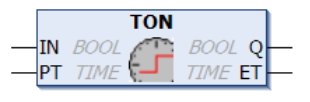
\includegraphics[width=0.4\textwidth]{images/BlockschaltbildTON.png}
		\caption{Blockschaltbild des Bibliotheksfunktionsblocks \textrm{TON}. Auszug aus dem Beckhoff-Infosys.}
		\label{fig:BlockschaltbildTON}
	\end{center}	
\end{figure}

Der Eingang \textrm{IN} ist das Startsignal. Nach Ablauf der vorgegebenen Zeit durch den Eingang \textrm{PT} (Periodtime), wird der Ausgang \textrm{Q} auf \textrm{TRUE} oder \textrm{1} gesetzt. Der zweite Ausgang gibt die verstrichene Zeit \textrm{ET} (Elapsed Time) seit dem Startsignal wieder und behält den Wert der voreingestellten Zeit \textrm{PT} nach Erreichen der Periodendauer. Sobald \textrm{IN} auf \textrm{FALSE} gesetzt wird, wird die verstrichene Zeit \textrm{ET} zurückgesetzt. Dieses Verhalten ist im Zeit-Signal Diagramm \ref{fig:Zeitsignaldiagramm} widergespiegelt.

\begin{figure}[H]
	\begin{center}
		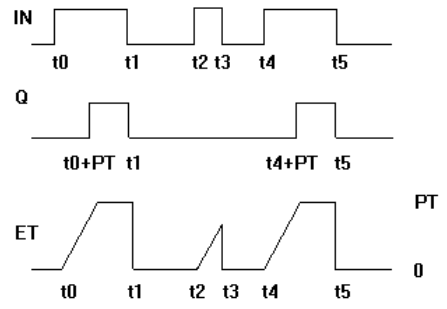
\includegraphics[width=0.4\textwidth]{images/ZeitSignalDiagramm.png}
		\caption[Zeit-Signal Diagramm des \textrm{TON} Bausteins.]{Zeit-Signal Diagramm des Bibliotheksfunktionsblocks \textrm{TON}.  Auszug aus dem Beckhoff-Infosys.}
		\label{fig:Zeitsignaldiagramm}
	\end{center}	
\end{figure}


Aufgerufen wird ein Bibliotheksfunktionsblock, wie jeder Funktionsblock durch Deklarierung im Deklarationsteil und Funktionsaufruf im Programmteil, siehe Listing \ref{lst:FBTON}.

\lstinputlisting[caption= Aufruf eines \textrm{TON} Funktionsblocks in einem Programm., label = lst:FBTON, style=ST]{Code/FBTON.txt}

\textbf{Targetsystems}

Bei der Entwicklung kann zum Programmtest mit virtuellen Inbetriebnahmen der Entwicklungsrechner verwendet werden. Im Betrieb  soll die Programmabarbeitung jedoch auf einem IPC erfolgen. Damit bei der Inbetriebnahme Anpassungen im Steuerprogramm möglich sind, kann der IPC als Zielsystem  (eng. Targetsystem) in TwinCAT  gewählt werden, um somit die Codeänderungen am PC auf dem IPC zu kompilieren. Dies ist möglich indem eine Netzwerkroute vom Entwicklungs-PC zum IPC errichtet wird. Die Route wird über die IP-Adresse erstellt und arbeitet mit dem ADS Protokoll \cite{InfosysADS}. Eine detaillierte Anleitung für das Anlegen einer Route finden Sie unter \cite{InfosysZielsystem}. Um Fehler zu vermeiden müssen vor einem Verbindungsversuch folgende Punkte beachtet werden.

\begin{itemize}
	\item[1.] Die Adapteroptionen der Ethernet-Verbindung darf nur das Internetprotokoll, Version 4 (TCP/IPv4) verwenden. IPv6 muss deaktiviert sein.
	\item[2.] Es ist zu überprüfen ob der zu verbindende IPC eine statische oder dynamische IP-Adresse verwendet. Bei Verwendung einer dynamischen IP-Adresse muss der Entwicklungs-PC ebenfalls auf eine dynamische Adressierung eingestellt sein. Bei statisch vergebener IP-Adresse des IPC's muss der Entwicklungs-PC das selben Subnetz verwenden.  (Beispiel: IP IPC: 192.168.10.01; IP PC: 192.168.10.02; bei gleichbleibender Subnetzmaske: 255.255.255.0;)
	\item[3.] TwinCAT Runtime Mode muss sich im \textrm{Konfig Mode} befinden.
\end{itemize}

\textbf{Einführungsaufgabe - Blinklicht}

Als Einführungsaufgabe in das Fachgebiet der SPS-Programmierung soll ein Blinklicht entworfen werden. Dieses Licht soll durch eine steigende Flanke eines Eingangs gestartet und bei erneuter Flanke ausgeschaltet werden. Die Flankenerkennung erfolgt über einen Trigger FB \textrm{R\_TRIG}, aus Abbildung \ref{fig:R-Trig}, um steigende Flanken zu erkennen. D.h. sobald der Eingang \textrm{CLK = TRUE}  wird, wird der Ausgang \textrm{Q = TRUE}. Jede weitere Ausführung des FB gibt \textrm{Q = FALSE} zurück, bis eine fallende und erneut eine steigende Flanke auftreten.   

\begin{figure}[H]
	\begin{center}
		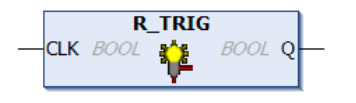
\includegraphics[width=0.4\textwidth]{images/R_Trig.png}
		\caption{Blockschaltbild des \textrm{R\_Trig} Funktionsbausteins. Auszug aus dem Beckhoff-Infosys.}
		\label{fig:R-Trig}
	\end{center}	
\end{figure}

Das Blinklicht kann durch einen \textrm{TON} FB, siehe Abbildung \ref{fig:BlockschaltbildTON}, erzeugt werden. Dazu wird der negierte Ausgang \textrm{Q}, mit dem Startsignal \textrm{bBlink}, durch ein logisches Und verknüpft und als Eingang \textrm{IN} am FB verwendet. Dadurch entsteht ein periodisches Sägezahnsignal durch \textrm{ET}, siehe Abbildung \ref{fig:Blinklichtsignal}. 

\begin{figure}[H]
	\begin{center}
		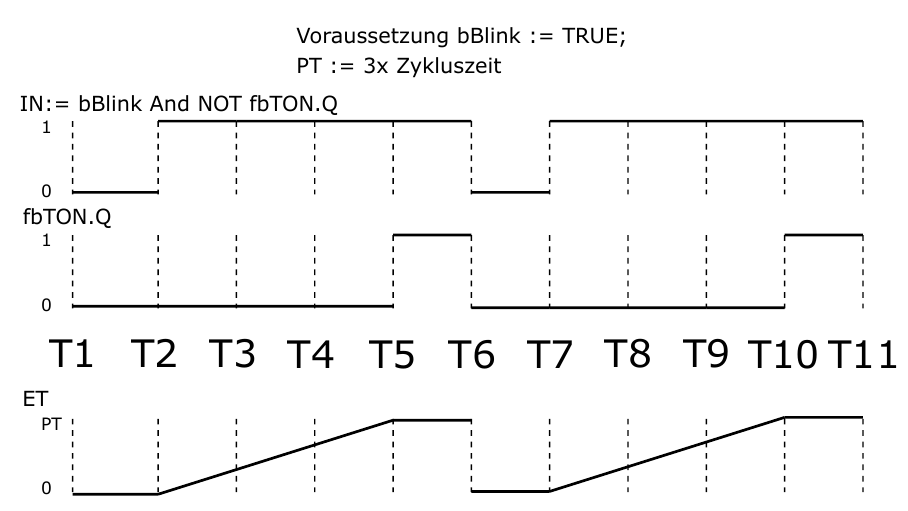
\includegraphics[width=0.8\textwidth]{images/Blinklicht_Zeit_Signal_Diagramm.png}
		\caption{Zeit-Signaldiagramm der Blinklichtsteuerung mit einem \textrm{TON}.}
		\label{fig:Blinklichtsignal}
	\end{center}	
\end{figure}

Das eigentliche Blinksignal kann nun aus dem Signal \textrm{ET} erzeugt werden, indem eine Abfrage implementiert wird, siehe Listing \ref{lst:EinfuehrungsbeispielFunktionsblock} Programmteil \textrm{BlinkPeriode = PT}, in welchem das Blinksignal \textrm{FALSE} ist, wenn \textrm{ET} kleiner \textrm{PT/2} ist und \textrm{TRUE}, wenn \textrm{ET} größer \textrm{PT/2} ist. Zuvor muss noch der Einschaltzustand definiert werden. Dies geschieht im Programmteil \textrm{Flankenabfrage}. Wenn eine Flanke am Signal \textrm{bIN} ankommt, wechselt die Variable \textrm{bBlink} ihren bool'schen Wert.

\lstinputlisting[caption=Funktionsbaustein zur Blinklichtsteuerung durch Flankensignal., label = lst:EinfuehrungsbeispielFunktionsblock, style=ST]{Code/Einfuehrungsbeispiel.txt}

Um den Funktionsbaustein \textrm{FB\_BlinkBsp} auszuführen, muss dieser im Programm \textrm{MAIN} aufgerufen werden und mit den richtigen Signalen der \textrm{IFC\_HW} verknüpft werden. Programm wird in Listing \ref{lst:EinfuehrungsbeispielFunktionsblock-MAIN} gezeigt.

\lstinputlisting[caption=Übergeordnetes Programm mit Aufruf des \textrm{FB\_BlinkBsp}., label = lst:EinfuehrungsbeispielFunktionsblock-MAIN, style=ST]{Code/Einfuehrungsbeispiel_MAIN.txt}

\subsection{Prozesszustandsbeschreibung}

Die beiden hier besprochenen Prozessbeschreibungsvarianten dienen der grafischen Darstellung von ansonsten verbal beschriebenen Prozessen. Einsatz finden diese Beschreibungen bei der Programmerstellung, Inbetriebnahmen und Fehlersuche. Mit Hilfe einer richtig erstellten Prozessbeschreibung, ist die Lösung der entsprechenden Steueraufgabe quasi gefunden. 

\subsubsection{Ablauf-Funktionsplan}

Der Ablauf-Funktionsplan ist geeignet für Prozesse mit unterscheidbaren Aktionen, die ereignis- oder zeitgesteuert in Reihen- oder auch Parallelfolge ablaufen. Er stellt nur grafische Elemente für eine Ablaufbeschreibung zur Verfügung, welche als Steuerzustände mit entsprechenden Aktionen und Übergangsstellen mit entsprechenden Bedingungen ausgeführt sind. Die Einteilung der Steuerzustände und Übergasstellen ist die eigentliche Herausforderung bei der Anwendung dieser Methode und bedarf Übung und Erfahrung. Der Ablauf-Funktionsplan soll dabei das Denken während der Entwurfsphase der Anlage unterstützen. In Abbildung \ref{fig:Ablauf-Funktionsplan} ist ein einfacher Ablauf, mit drei Zuständen drei Übergängen und einer Rückführschleife für den Neustart des Ablaufes, dargestellt. 

\begin{figure}[H]
	\begin{center}
		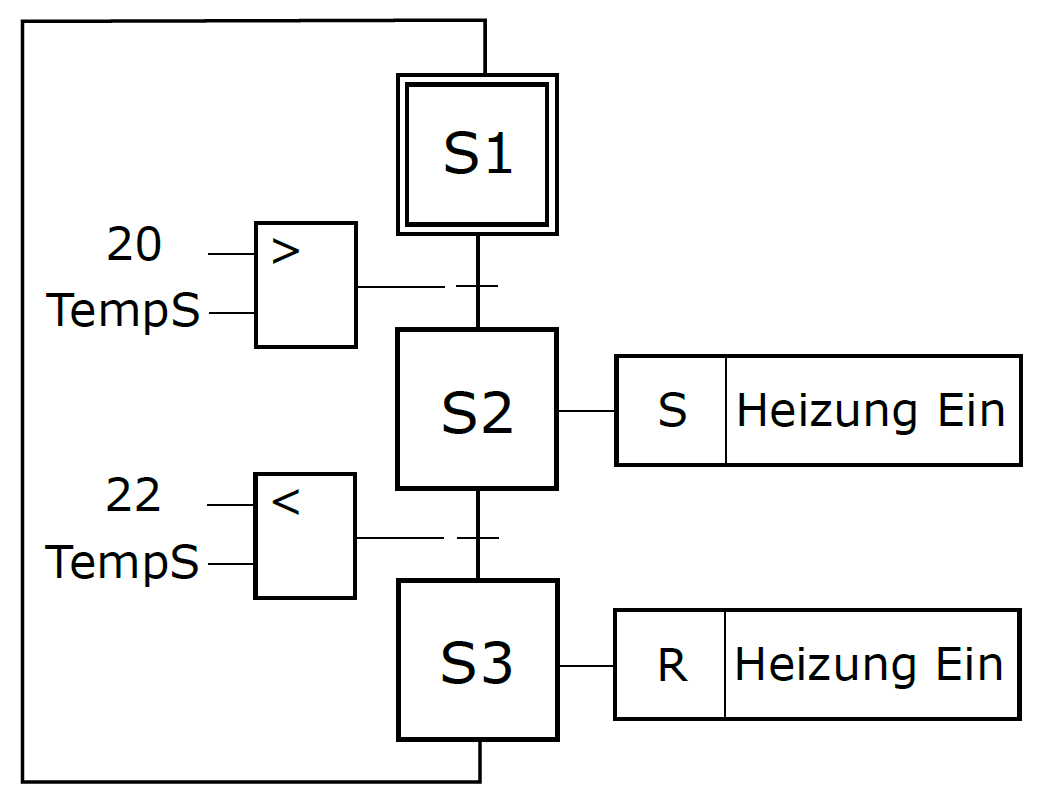
\includegraphics[width=0.4\textwidth]{images/AblaufFunktionsplan.png}
		\caption{Ablauf-Funktionsplan einer Heizung mit Zweipunktregelung.}
		\label{fig:Ablauf-Funktionsplan}
	\end{center}	
\end{figure}


\subsubsection{Zustandsübergangsdiagramm} \label{sec:Zustandsgraphen}

Sobald Prozessabfolgen keinen zwangsläufigen schrittweisen Ablauf mehr besitzen, ist die Anwendung des Ablauf-Funktionsplan nur schwer möglich. Als alternative Beschreibungsmethode kann hier ein Zustandsübergangsdiagramm verwendet werden. Dies beschreibt eine Zustandsmaschine, zu eng. State Machine genannt und ermöglicht es aus jedem Zustand in jeden anderen Zustand zu wechseln, sofern dies für den Ablauf des Prozesses erforderlich ist. Jeder Zustand wird als Kreis mit eindeutiger Nummer dargestellt, siehe Abbildung \ref{fig:Zustandsdiagramm}. Die Transitionen werden im Diagramm durch Pfeile dargestellt, wobei aus einem Zustand mehrere Übergange wegführen bzw. hinführen können. Ähnlich wie bei Ablauf-Funktionsdiagrammen, können in den Zuständen und Transitionen Aktionen durchgeführt werden, welche ausgeführt werden, bis der Zustand verlassen bzw. die Transition vollendet ist. 

Da es in dieser Prozessbeschreibung mehrere Transitionen pro Zustand geben kann und diese auch gleichzeitig zutreffen können ist eine Priorisierung der Übergänge notwendig. Dies kann durch aufsteigende Nummerierung der Pfeile festgelegt werden. Wobei 1 die höchste Priorität ist. 

Um beim Start der State Machine aus einem definierten Zustand zu starten, wird dieser durch einen gestrichelten Pfeil aus dem Nichts gekennzeichnet. Dieser Zustand wird normalerweise mit der Zustandsnummer 0 nummeriert. 

Bei Störungen oder ähnlichem kann es notwendig sein, Sprunghaft den Zustand zu wechseln. Der Zielzustand, z.B. Fehlerzustand, muss von allen Zuständen aus erreichbar sein. Diese Art der Transition wird als Any-Transition bezeichnet und mit einem durchgehenden Pfeil aus dem Nichts in den Zustand markiert. Diese Transition sollte immer mit höherer Priorität als die Transitionen zwischen den Zuständen versehen sein. Um nach Aufhebung der Störung wieder mit dem Prozess fortfahren zu können, gibt es Return-Transitionen, welche durch einen Merker den Zustand vor der Any-Transition gespeichert haben. Die Priorität dieser Transition muss nicht zwangsläufig höherer ausfallen wie die der allgemeinen Schrittkette. \cite{Wellenreuther.2015}   

\begin{figure}[H]
	\begin{center}
		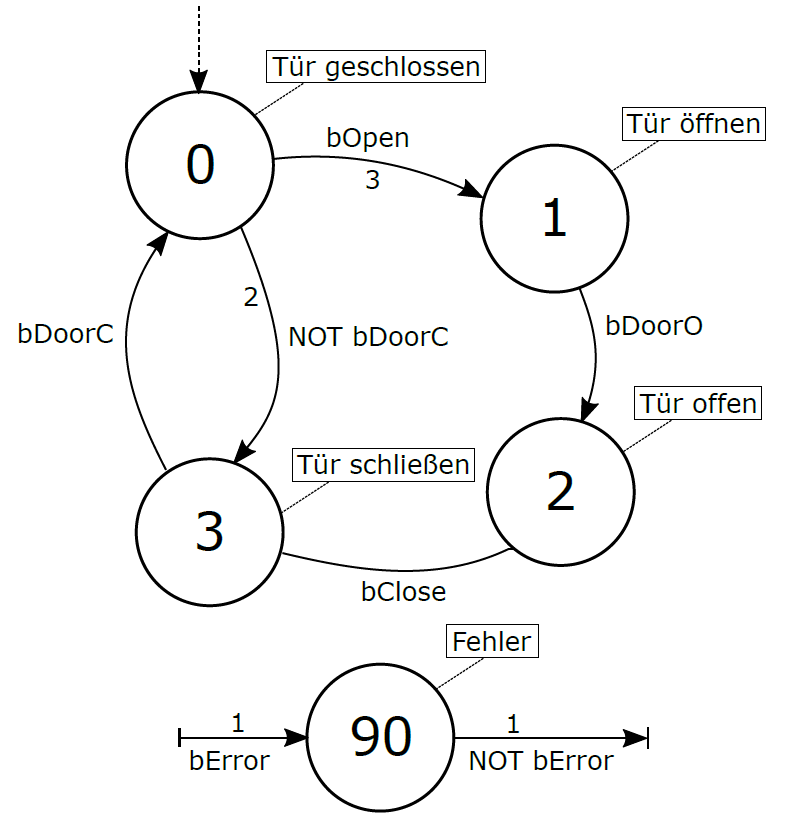
\includegraphics[width=0.6\textwidth]{images/Zustandsuebergangsdiagramm.png}
		\caption[Beispielhafter Zustandsgraph einer Maschinentür.]{Beispielhaftes Zustandsübergangsdiagramm für eine Türsteuerung mit Näherungssensoren zur Detektion der Türposition. Zwei Signale zum öffnen bzw. schließen und automatischer Schließfunktion beim Start der Steuerung.}
		\label{fig:Zustandsdiagramm}
	\end{center}	
\end{figure}


\subsection{Virtuelle Inbetriebnahme}

Die virtuelle Inbetriebnahme (VIB) von Produktionsanlagen ist eine fortschrittliche Methode, die es ermöglicht, den Inbetriebnahmeprozess virtuell durchzuführen, bevor physische Anlagenkomponenten real vorhanden sind. Dieser Ansatz bietet mehrere Vorteile und ist in verschiedenen Industriezweigen weit verbreitet.

Sie bezieht sich auf die Simulation und Überprüfung von Anlagenprozessen und -steuerungen in einer virtuellen Umgebung, noch bevor die tatsächlichen Anlagenkomponenten physisch existieren. Durch den Einsatz von Software-Tools werden alle relevanten Aspekte einer Produktionsanlage, einschließlich Steuerungen, Sensoren, Aktoren und mechanischer Komponenten, in einer virtuellen Umgebung nachgebildet. Die virtuelle Inbetriebnahme ermöglicht die frühzeitige Erkennung von Fehlern und Problemen im Steuerungs- und Automatisierungssystem, noch bevor die Anlage gebaut oder installiert wird. Dies trägt dazu bei, teure Nachbesserungen in späteren Phasen zu vermeiden. Durch die Simulation können Steuerungsprogramme optimiert und getestet werden, um sicherzustellen, dass sie effizient und fehlerfrei arbeiten. Dies trägt dazu bei, die Inbetriebnahmezeit vor Ort zu reduzieren. Des weiteren ermöglicht diese Entwicklungsmethode auch Schulungen und Training für das Bedienpersonal während der Umsetzungsphase der Anlage, um sie auf den Betrieb vorzubereiten, bevor diese physisch vorhanden ist.

Einsatz findet diese Methode in verschiedenen Branchen, darunter die Automobilindustrie, die Luft- und Raumfahrt, die Prozessindustrie und die Fertigung, um nur einige Beispiele zu nennen. In diesen Branchen werden die bestehenden Product Lifecycle Management (PLM)-Systemen eng mit der VIB verbunden, um eine nahtlose Integration zwischen der virtuellen und realen Umgebung zu gewährleisten. Dadurch können Fehler frühzeitig identifiziert und behoben und Steuerungsprogramme optimiert werden.

Insgesamt ermöglicht die virtuelle Inbetriebnahme eine effiziente und risikoarme Entwicklung, Validierung und Inbetriebnahme von Produktionsanlagen, was zu einer höheren Zuverlässigkeit und Effizienz in der realen Umgebung führt.

Die Abkürzungen MiL, SiL, HiL und AT configuration stehen im Zusammenhang mit verschiedenen Phasen der virtuellen Inbetriebnahme und beziehen sich auf unterschiedliche Testebenen. Hier sind die Erklärungen für jede Abkürzung beschrieben und grafisch dargestellt in Abbildung \ref{fig:VirtuelleInbetriebnahme}.

\begin{figure}[H]
	\begin{center}
		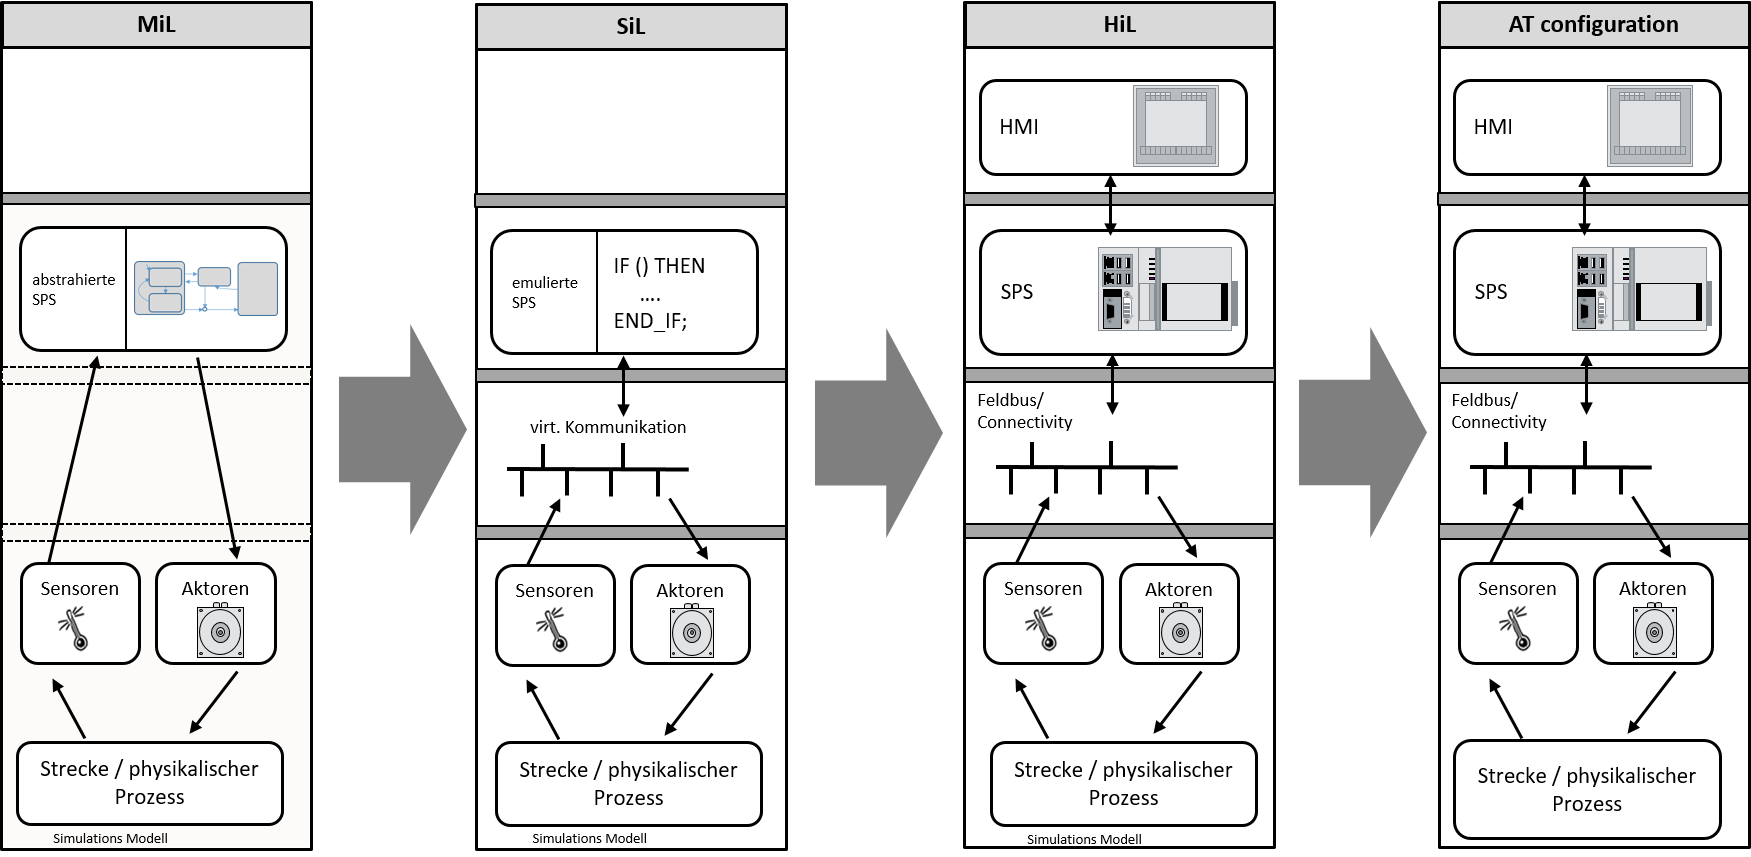
\includegraphics[width=0.9\textwidth]{images/Virtuelle Inbetriebnahme.png}
		\caption{Entwicklungsphasen unter der Verwendung von virtueller Inbetriebnahme.}
		\label{fig:VirtuelleInbetriebnahme}
	\end{center}	
\end{figure}

\textbf{MiL - Model-in-the-Loop}

MiL bezieht sich auf die Testebene, bei der das Modell der Steuerungssoftware in einer Simulationsumgebung getestet wird, noch bevor die reale Hardware verfügbar ist. Hier wird das Simulationsmodell des Steuerungssystems verwendet, um die Funktionalität und das Verhalten der Software zu überprüfen.

\textbf{SiL - Software-in-the-Loop}

Bei SiL wird die Testebene erreicht, wenn die Software in einer Simulationsumgebung auf ihre Funktionalität überprüft wird. Hierbei wird das reale Steuergerät oder die Hardware-Schnittstelle simuliert, um die Wechselwirkung zwischen der Software und der Hardware zu testen.

\textbf{HiL - Hardware-in-the-Loop}

HiL bezieht sich auf die Testebene, bei der die reale Hardware in einer physikalischen Simulation integriert wird. Hier wird die Steuerungssoftware mit der Simulierten Hardware verbunden, um das Zusammenspiel in einer realistischen Umgebung zu überprüfen. Dies ermöglicht eine detaillierte Verifikation der Steuerungssoftware in Bezug auf die physischen Hardwarekomponenten.

\textbf{AT configuration - Acceptance Test Configuration} 

AT configuration bezieht sich auf die Konfiguration der Akzeptanztests. In dieser Phase wird die virtuelle Inbetriebnahme genutzt, um sicherzustellen, dass das Gesamtsystem, bestehend aus Hard- und Software, die gestellten Anforderungen erfüllt. Dies ist die letzte Stufe vor der physischen Inbetriebnahme der Anlage.

Zusammengefasst spiegeln diese Abkürzungen die schrittweise Entwicklung und Verfeinerung der virtuellen Inbetriebnahme wider, beginnend mit dem Modelltest (MiL), über den Softwaretest (SiL), den Hardwaretest (HiL) bis hin zur Akzeptanzprüfung (AT configuration) des Gesamtsystems. Diese Schritte helfen dabei, Fehler frühzeitig zu erkennen, die Software zu optimieren und die Gesamtzuverlässigkeit der Anlage sicherzustellen, bevor diese physisch aufgebaut wird.
  


\subsection{Basisaufgaben}

Diese Beispiele dienen zur Erhöhung des Verständnisses der bisherigen Inhalte und sollen direkt Einblicke in eine praktische Umsetzung geben. Im ersten Beispiel wird die Vereinzelung der Teaching Factory beschrieben. Das zweite Beispiel dient der Erstellung einer Betriebszustandsanzeige in Form einer Ampelleuchte. Bitte beachten Sie, dass eine zeitnahe Umsetzung von großem Vorteil ist, da die hier besprochenen Inhalte in den nächsten Kapiteln verstanden werden müssen. 

\subsubsection{Vereinzelung - 10 Punkte}

Die Vereinzelung ist der erste Arbeitsschritt im Abfüllprozess der Teaching Factory. Die hier gezeigte Implementierung und das zu Grunde liegende Konzept können mit wenigen Anpassungen für alle Vereinzelungsprozesse verwendet werden. Zur Umsetzung dieses Beispiel wird der Automatisierungsprozess in sechs Schritte unterteilt. Durch diese Vorgangsweise können auch alle weiteren Prozesse automatisiert werden. Die einzelnen Schritte sind:

\begin{itemize}
	\item[1] Prozessschema erstellen (Anlagendesign)- dabei soll die allgemeine Funktionsweise bildlich dargestellt und alle Komponenten mit Namen versehen werden. Der Prozess kann wörtlich beschrieben werden. 
	\item[2.] Ablaufdiagramm erstellen (Anlagenablauf)- Aus dem Prozessschema soll ein Ablauf definiert werden. Hier ist speziell auf die Reihenfolge und Prozessverzweigungen Rücksicht zu nehmen. Durch die Namensvergebung der Komponenten ist eine eindeutige Zuordnung zwischen Prozessschema und Ablaufdiagramm vorhanden.
	\item[3.] Sensor- und Aktuatorauswahl (Anlagenauslegung)- durch die Auswahl der Sensoren und Aktuatoren sind die notwendigen Elektrischen Signale bekannt. 
	\item[4.] Auswahl der E/A-Geräte (Anlagensteuerung) - mit der Signalliste der Sensoren und Aktuatoren können passende E/A-Geräte definiert werden. 
	\item[5.]  SPS-Programmierung (Anlagenprogrammierung)- mit Hilfe des Ablaufdiagramms und der Signalliste kann jeder Schritt im Prozess mit den dazugehörenden Signalzuständen beschrieben und in ein Zustandsübergangsdiagramm überführt werden. Dieses Diagramm dient zu Programmierunterstützung.
	\item[6.] Prozess und Programmoptimierung (Anlagenoptimierung)- Der Prozess und das Programm können validiert und optimiert werden nachdem der Prozess automatisiert wurde. 	 
\end{itemize} 

\textbf{1. Prozessschema erstellen (Anlagendesign)}

Ein Schema der Vereinzelung ist in Abbildung \ref{fig:Schemata_Vereinzelung} dargestellt und besteht aus dem vertikalen Speicherbereich - somit wird die Teileförderung durch Gravitation umgesetzt -, der Vereinzelungskammer - abgegrenzt durch die zwei Schleusen - und den notwendigen Sensoren für die Teileerkennung. Zusätzlich ist ein Abtransportsystem, in Form eines Förderbandes, eingezeichnet. Dieses kann in anderen Anlagen auch durch unterschiedliche Komponenten, wie z.B. eine Rutsche, ersetzt werden.


\begin{figure}[H]
	\begin{center}
			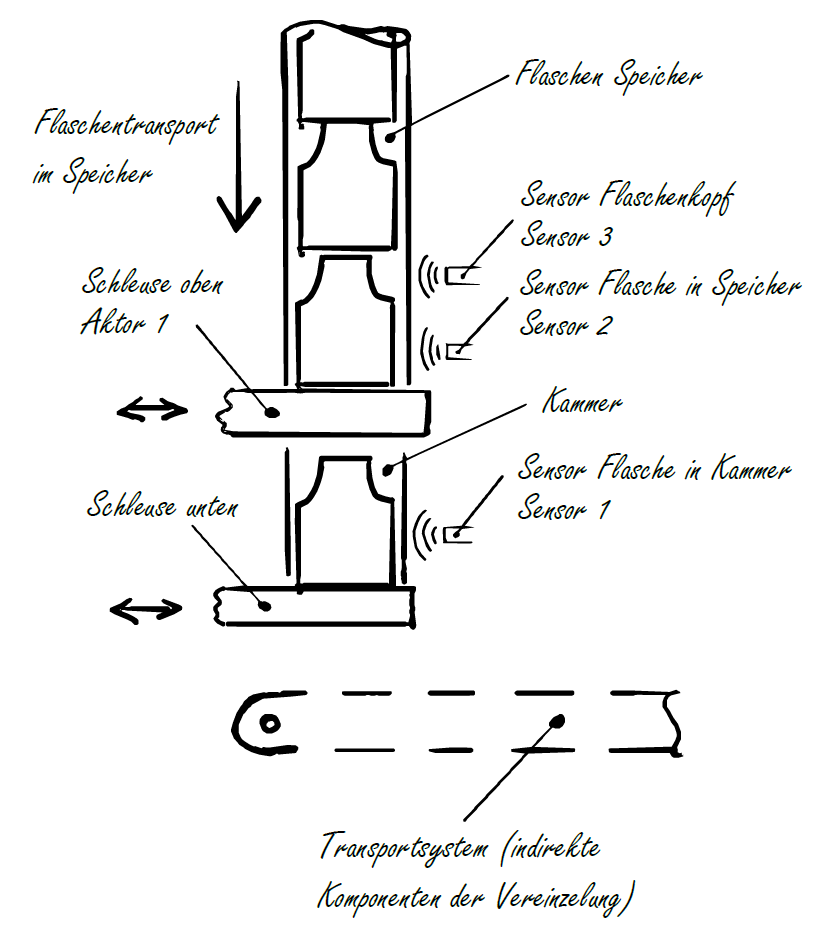
\includegraphics[width=0.6\textwidth]{images/Schemata_Vereinzelung.png}
			\caption{Schema der Vereinzelung.}
			\label{fig:Schemata_Vereinzelung}
		\end{center}	
\end{figure}

Der Prozessablauf kann wie folgt Formuliert werden. Im Ausgangszustand wird angenommen, dass der Speicher manuell mit Flaschen befüllt wurde und dass beide Schleusen in geschlossener Position stehen.  Die Sensoren "Flaschenkopf" und "Flasche in Speicher" detektieren eine richtig positionierte Flasche im Speicher durch die Signalkombination "Flaschenkopf" = FALSE und "Flasche in Speicher" = TRUE.
Somit kann die erste Schleuse geöffnet werden bis der Sensor "Flasche in Kammer" eine Flasche erkennt. Im Anschluss kann die obere Schleuse gleich wieder geschlossen werden. Sobald die Schleuse oben geschlossen ist, kann die untere Schleuse geöffnet werden und wieder geschlossen, wenn die Flasche die Kammer verlassen hat. 
Somit ist der Ausgangszustand wieder erreicht und der Prozess kann erneut beginnen.    

\textbf{2. Ablaufdiagramm erstellen (Anlagenablauf)}

Um die Überführung des Prozesses von menschlicher Sprache in Maschinensprache zu beginnen, bietet es sich an, ein Ablaufdiagramm zu erzeugen. Diese ist in Abbildung \ref{fig:Ablaufdiagramm} dargestellt und beinhaltet 3 Symboltypen:

\begin{itemize}
	\item Start/Stop des Prozesses (rechteckig),  \hspace{2cm} 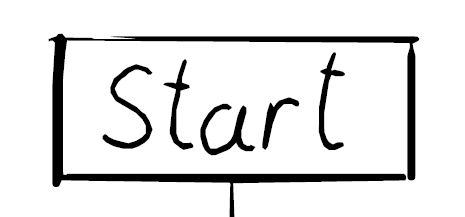
\includegraphics[ height =30 pt]{images/Start.png}
	\item Aktionen bzw. Arbeitsschritte (Oval) und   \hspace{1,5cm} 
\includegraphics[ height =30 pt]{images/Aktion.png}
	\item Abfragen bzw. Verzweigungen (Raute).  \hspace{2cm} 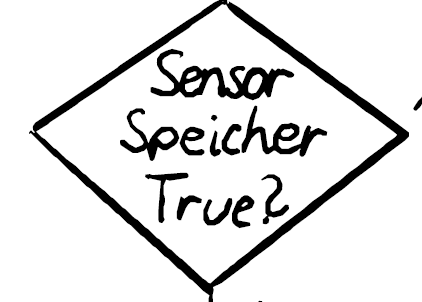
\includegraphics[ height =40 pt]{images/Abfrage.png}
\end{itemize}

Für die meisten Ablaufdiagramme sind diese Symbole ausreichend. Zusätzliche Symbole, für zum Beispiel Datenspeicherung oder Meldungen, können bei bedarf ergänzt werden. 

\begin{figure}[H]
	\begin{center}
		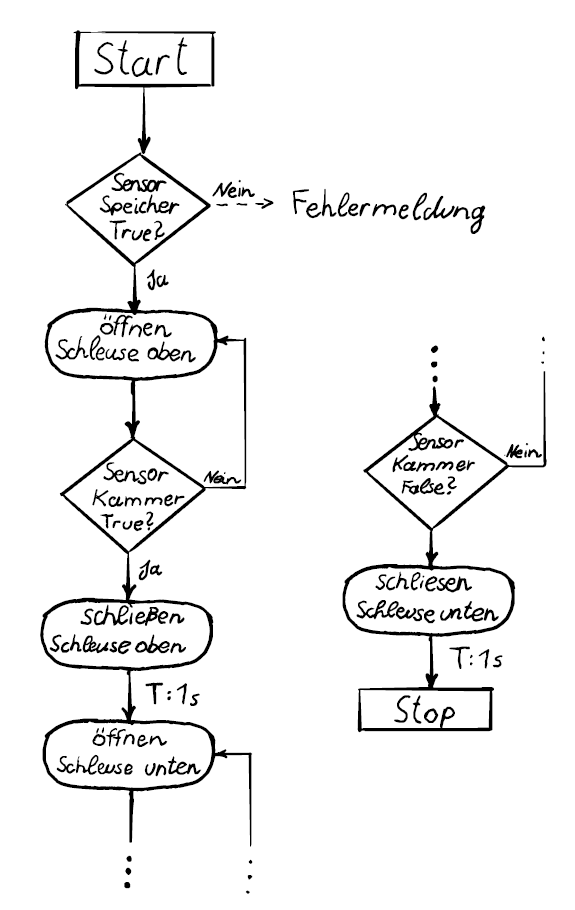
\includegraphics[width=0.55\textwidth]{images/Ablaufdiagramm_Vereinzelung.png}
		\caption[Ablaufdiagramm der Vereinzelung.]{Ablaufdiagramm der Vereinzelung. Dieses Arbeitsblatt muss nicht durch Zeichentools erstellt werden, einfache Handskizzen sind ausreichend.}
		\label{fig:Ablaufdiagramm}
	\end{center}	
\end{figure}

Es ist zu sehen, dass der Vereinzelungsprozess aus vier Arbeitsschritten besteht. Diese ergeben sich daraus, dass jede Schleuse einmal auf und zu gemacht werden muss. Eine Zustandsabfrage ist dreimal vorhanden, wobei die beiden letzteren in den vorherigen Arbeitsschritt zurückgehen. Somit ist in diesem Fall keine Prozessverzweigung vorhanden, sondern ein Arbeitsschritt wird so lange ausgeführt, bis eine Änderung der Abfrage geschieht. Dies bedeutet beim Einsatz einer SPS mit zyklischer Programmlaufzeit, dass dieser Arbeitsschritt über mehrere Zyklen ausgeführt wird. 
Die erste Abfrage vollzieht hingegen eine Art Prozessabzweigung bei der eine Fehlermeldung für nicht vorhandene Flaschen angezeigt wird. Diese Fehlerbehandlung wird, zur Vereinfachung des Programmierens, in weitere Folge vernachlässigt und später im Kapitel \ref{cpt:Fehlerbehandlung} wieder aufgenommen. Dort wird ersichtlich, dass eine Mischung von Prozessprogramm und Fehlerbehandlungsprogrammen zu einem unübersichtlichen Code führt und es somit einer anderen Vorgehensweise bedarf.  

\textbf{3. Sensor- und Aktuatorauswahl (Anlagenauslegung)}

Die Umsetzung des Prozesses durch ein technisches System erfordert die Auswahl geeigneter Wirkprinzipien. Bei der Flaschenförderung im Speicher wird in diesem Fall die Förderung durch Gravitation realisiert, wobei alternative Methoden wie die Verwendung von Förderbändern ebenfalls möglich sind. Die Varianten der Flaschenförderung erfordert jedoch eine klare Unterscheidung zwischen aktiven und passiven Fördersystemen, da dies einen Einfluss auf die erforderlichen E/A-Geräte hat.

Die Separation der Flaschen wird durch zwei Schleusen realisiert, doch auch ein Drehtisch mit einer Ausnehmung für eine Flasche kann effektiv genutzt werden. Sowohl lineare als auch rotierende Antriebe können als Aktuatoren für die Separation dienen. Es gibt zahlreiche Ausführungsvarianten für beide Kategorien, die mit den gängigen Energieversorgungsformen der Pneumatik, Hydraulik oder Elektrik realisiert werden können.

Die Flaschenförderung nach der Vereinzelung kann, ähnlich wie bei der Speicherlösung, entweder durch eine rutschfähige Bahn als passives Element oder durch ein Förderband mit einem entsprechenden Aktor als aktives Element implementiert werden.

Die Detektion von Flaschen bietet ebenfalls diverse Möglichkeiten, bei denen unterschiedliche Sensoren einsetzbar sind oder sogar auf Sensoren verzichtet werden könnte. Letzteres würde jedoch die Steuerbarkeit der Anlage erheblich einschränken. Insgesamt zeigt sich, dass die Umsetzung des Prozesses durch die Auswahl verschiedener Wirkprinzipien und Aktuatoren sowie die Anwendung unterschiedlicher Energieversorgungsformen eine facettenreiche Gestaltung der Anlage ermöglicht. In Tabelle \ref{tab:SensorAktorListe} sind die gewählten Sensoren und Aktoren für die Vereinzelung nach dem Schema aus Abbildung \ref{fig:Schemata_Vereinzelung} aufgelistet.




\textbf{4. Auswahl der E/A-Geräte (Anlagensteuerung)}

Durch die Anlagenauslegung sind die Anzahl und Arten der notwendigen Steuersignale definiert. Hier geht es nun darum, die passenden E/A-Geräte für die Signale zu bestimmen. In diesem Beispiel handelt es sich nur um digitale Ein- und Ausgänge somit ist die Auswahl relative einfach. Die Sensor Signale können mit einer digitalen Eingangsklemme, mit z.B vier Kanälen, in die Steuerung integriert werden. Da es sich zusätzlich um nicht mechanische Schalter handelt, kann auf den Prellschutz in der Eingangsklemme verzichtet werden. Wie in Tabelle \ref{tab:EAGeraete} zu sehen ist, wird jedoch eine 8-Kanal Klemme verwendet, da es in den weiteren Komponenten der Teaching Factory zusätzliche digitale Eingangssignale gibt, welche auf diese Klemme angeschlossen werden.\\
Bei den Bipolaren \SI{24}{\volt} Signalen ist die Auswahl jedoch etwas komplexer. Während des Ausfahrens der Zylinder muss Leitung A mit \SI{24}{\volt} versorgt und Leitung B an \SI{0}{\volt} angeschlossen sein. Um den Zylinder wieder einfahren zu können muss eine Umpolung in den Leitungen A und B geschehen. Diese Verhalten kann durch einer Relaisschaltung mit vier Relais umgesetzt werden, siehe Abbildung \ref{fig:Relaisschaltung}. 

\begin{figure}[H]
	\begin{center}
		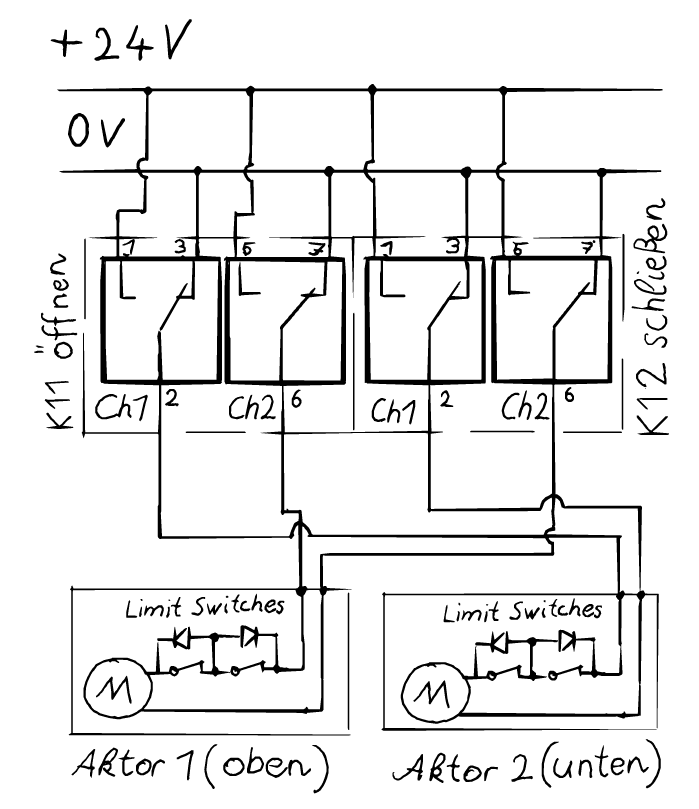
\includegraphics[width=0.5\textwidth]{images/Relaisschaltung.png}
		\caption{Aufbau der Relaisschaltung für die Schleusen EZylinder der Vereinzelung.}
		\label{fig:Relaisschaltung}
	\end{center}	
\end{figure}




Damit die richtigen Kanäle angesprochen werden muss aus dem Schaltplan eine Zuweisung der Variablen entnommen werden. Wie in der oberen Abbildung \ref{fig:Relaisschaltung} zu sehen ist, sind die Kanäle 1 und 2 der beiden Klemmen EL 2652 mit den Aktuatorenanschlüssen zu verdrahten. Dadurch bekommt der Kanal 1 Klemme 11 (K11) die Funktion den zweiten Aktor zu öffnen, wenn das Relais geschallten wird. Voraussetzung ist dabei, dass Kanal 1 Klemme 12 (K12) nicht betätigt und somit das Relais auf \SI{0}{V} durchschaltet. Gleiches gilt für Aktor 1 und dem Kanal 2 an der Klemme 11 und 12. Die Kanalvergabe aller Klemmen ist in Tabelle \ref{tab:Signalliste} ersichtlich. Ebenfalls werden die DI's für die Klemme EL1018 gelistet. Diese Prozesssignale und alle weiteren Prozesssignale der Teaching Factory werden innerhalb der SPS-Steuerung in einer Globalen Variablen Liste \textrm{IFC\_HW} zusammengefasst. Dies bildet das Hardware Interface, welches die Signale der Anlage mit den Variablen des Steuerungsprogramms verknüpft.  





\textbf{5. SPS-Programmierung (Anlagenprogrammierung)}

Der Prozess der Vereinzelung soll durch einen Funktionsblock implementiert werden. Dieser ist so aufgebaut, dass er für mehrere Vereinzelungen einsetzbar ist. Somit werden die E/A-Signale aus Tabelle \ref{tab:Signalliste} nicht Eins zu Eins als E/A-Variablen gehandhabt. Stattdessen werden die Schaltzustände der Ezylinder durch zwei bool'sche Variablen \textrm{bGate1} und \textrm{bGate2} ersetzt. Die Schleusen sind beim Zustand \textrm{False} und \textrm{False} geschlossen und geöffnet bei \textrm{True} und \textrm{True}. Die Zuordnung, zu den globalen Variablen der \textrm{IFC\_HW} und somit den tatsächlichen Relaiszuständen, erfolgt nach Aufruf des Funktionsblocks durch eine weitere Funktion im übergeordneten, anwendungsspezifischen Hauptprogramms.\\
Damit der Prozess wie im Ablaufdiagramm dargestellt funktionieren kann, müssen für jeden Arbeitsschritt die Ausgangszustände definiert werden. Damit dieser Zustand auch im richtigen Moment wechselt, müssen die Signale den Abfragen zugewiesen werden. Diese Zuordnung der Zustände und Signale wird in Abbildung \ref{fig:ZustandSignalListe} dargestellt. Dabei wird ebenfalls eine Durchnummerieren nach Zustandswechsel vollzogen.  

\begin{figure}[H]
	\centering
	\def\svgwidth{250pt}
	\input{images/Zustand_Signal_Liste_V2.png_tex}
	\caption{Zuordnung der Signalzustände zu den einzelnen Zuständen.}
	\label{fig:ZustandSignalListe}
\end{figure}

Nachdem die Signalzustände und Arbeitsschritte verknüpft sind, kann das Zustandsübergangsdiagramm erstellt werden. Mit Hilfe dieses Diagramms ist die Implementierung der Prozessschrittkette in Strukturierten Text (ST) einfach umsetzbar. Abbildung \ref{fig:ZustandsdiagrammVereinzelung} zeigt das Zustandsübergangsdiagramm. Da es sich hierbei um ein einfaches Beispiel handelt und sich die Zustandsvariablen auf zwei bool'sche werte beschränken, können diese in die Zustände S1 bis S5 eingetragen werden. Bei komplexeren Systemen ist es oftmals übersichtlicher die Zustandsvariablen nur in der Zustandsliste anzuführen.

\begin{figure}[H]
	\begin{center}
		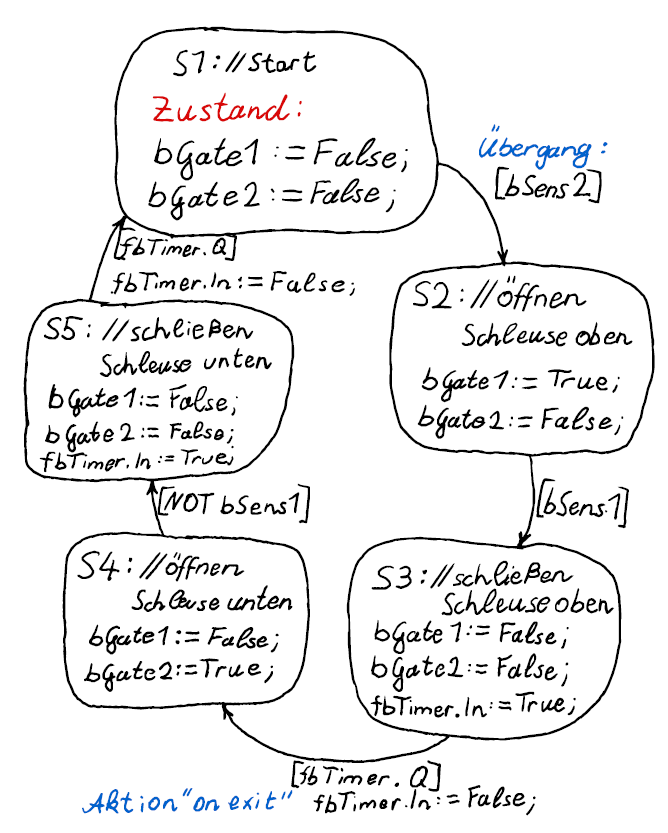
\includegraphics[width=0.55\textwidth]{images/Zustandsuebergangsdiagramm_Vereinzelung.png}
		\caption{Zustandsübergangsdiagramm der Vereinzelung mit Programmierhilfen.}
		\label{fig:ZustandsdiagrammVereinzelung}
	\end{center}	
\end{figure}

Die Programmüberführung aus dem Zustandsübergangsdiagramm in Strukturierten Text (ST) lässt sich durch die Verwendung einer CASE-Anweisung umsetzen. Diese Anweisung dient der Auswahl von 1-n unterschiedlichen Programmteilen. Die Auswahl beruht auf einer INTEGER Variable. Für das Programmieren einer State Machine kann die Zustandsnummer S1-Sn als Auswahlvariable verwendet werden. Im Programmteil werden die jeweiligen Signalzustände gesetzt. Um einen Zustand verlassen zu können, wird eine einfache IF-Anweisung geschrieben, welche die jeweiligen Eingangsvariablen der Übergangsbedingung abfragt. Sobald die Übergangsbedingung zutrifft, werden die Anweisungen  der IF-Abfrage, wie die "on exit" Aktionen gesetzt, z.B \textrm{fbTimer.In := False;} und es wird die Auswahlvariable  auf den nächsten Zustand der State Machine gesetzt. Als Beispiel wird der Zustand S1 betrachtet mit der Auswahlvariable \textrm{nState : INT := 1;}, siehe Listing \ref{lst:Programmueberfuehrung}. Der gesamte Code für das Beispiel der Vereinzelung ist in Listing \ref{lst:CodeVereinzelungDraft} im Anhang dokumentiert.

\lstinputlisting[caption=Beispiel zur Programmüberführung des Zustandsgraphen in ST mit CASE-Anweisung., label = lst:Programmueberfuehrung, style=ST]{Code/Programmueberfuehrung.txt}



 Da die Ausgänge dieses Funktionsblockes nicht ausreichen um die Relais anzusteuern, muss eine weiterer Funktionsbaustein erstellt werden, welche die Relaissignale nach Tabelle \ref{tab:Signalliste} ausgeben.  Aus dieser Tabelle  ergibt sich die Wahrheitstabelle in \ref{tab:Wahrheitstabelle} für einen Aktor. Eine Funktion kann hier nicht verwendet werden, da zwei Ausgangswerte benötigt werden. Dieser Funktionsbaustein dient dazu, dass die Ablaufsteuerung für allgemeine Vereinzelungen verwendet werden kann und die anwendungsspezifischen Signale in der übergeordneten Steuerung gesetzt werden. 




Aus dieser Tabelle kann die Funktion aus Listing \ref{lst:Relaisfunktion} erstellt werden. 

\lstinputlisting[caption=Funktionsblock für Relaissteuerung., label = lst:Relaisfunktion, style=ST]{Code/fbRCtrl.txt}


\textbf{6. Prozess- und Programmoptimierung (Anlagenoptimierung)}

Beim genaueren Betrachten des Steuerprogramms der Vereinzelung treten zwei ungünstige Verhaltensweisen auf. Erstens erfolgt die zyklische Vereinzelung der Flaschen ohne externe Kontrolle. Zweitens besteht die Möglichkeit, dass eine Flasche bei einer Fehlfunktion des Förderbandes in der unteren Schleuse stecken bleibt, was bei wiederholtem Auftreten zu Beschädigungen führen kann. Aus diesem Grund wird in Abbildung \ref{fig:VereinzelungOptimiert} eine optimierte Ablaufsteuerung vorgeschlagen. Diese beinhaltet zwei zusätzliche Eingangssignale, um die Vereinzelung zu initiieren und anschließend den eigentlichen Vereinzelungsprozess zu starten. Um das Risiko von Flaschenklemmungen zu minimieren, wird die Ablaufsteuerung um einen Sensor erweitert. Dieser Sensor, idealerweise ein Näherungssensor am ersten Abfüllplatz, soll die Flasche außerhalb der Kammer detektieren. Sobald die Flasche durch das Förderband diese Stelle erreicht, kann der Vereinzelungsprozess abgeschlossen werden. 

Eine zusätzliche Erweiterung dieses Zustandsgraphen bezieht sich auf die Betriebszustandsvariablen. Jeder Prozesszustand befindet sich in einem der definierten Betriebszustände, die beispielsweise als Off, Init, Ready, Production, Done, Error, Stop oder Setup festgelegt werden können. Diese Betriebszustände sind einheitlich für die gesamte Anlage, sowohl für die einzelnen Komponenten als auch für einzelne Aktoren und Sensoren, und dienen somit als standardisierte Schnittstelle zwischen übergeordneten und untergeordneten Steuereinheiten. Die Betriebszustände werden als Ausgang an eine übergeordnete Steuereinheit zurückgemeldet, wodurch der Gesamtprozess der Anlage gesteuert werden kann.  

Für den Fall, dass die Produktion gestoppt werden soll, kann das bEnable Signal entzogen werden und der Prozesszustand \textrm{0: Off} wird aktiviert. Der, auf diesem Zustandsdiagramm basierte, Funktionsblock ist im Anhang in Listing \ref{lst:CodeVereinzelungOpt} zu sehen.

\begin{figure}[H]
	\begin{center}
		\includegraphics[width=0.8\textwidth]{images/VereinzelungOptimiert.png}
		\caption[Optimierter Zustandsgraph der Vereinzelung.]{Optimiertes Zustandsdiagramm der Vereinzelung mit Enable und Execute Signalen, sowie Sensorerweiterung, um Flaschenklemmung zu verhindern. }
		\label{fig:VereinzelungOptimiert}
	\end{center}	
\end{figure}

Die vorgestellten Erweiterungen der Ablaufsteuerung können als ein allgemeines Framework für Funktionsbausteine auf den Ebenen Modul-, Prozess- und Hardware betrachtet werden. Kapitel \ref{sec:Ebenenmodell} wird detailliert aufzeigen, wie das Ebenenkonzept aufgebaut ist und welche Unterschiede zwischen den einzelnen Ebenen bestehen. Als Ergebnis dieser Erweiterungen ist festzustellen, dass alle Funktionsbausteine gleichartig angesteuert werden können und ein einheitliches Feedback liefern, wenn ein Prozess startbereit oder abgeschlossen ist. Diese Harmonisierung führt zu einem reduzierten Programmieraufwand. Darüber hinaus ermöglicht die Verwendung eines definierten Frameworks die Aufteilung der Programmierung auf mehrere Entwickler, ohne dass ein erheblicher Abstimmungsaufwand erforderlich ist.


\subsubsection{Betriebszustandsampel - 5 Punkte}

Die Betriebszustandsampel soll den allgemeinen Anlagenzustand wiedergeben und somit den Bedienern der Anlage direkt den Betriebszustand anzuzeigen. Damit die Ampel definierte Leuchtsignale anzeigt wird ein Funktionsbaustein benötigt. Die Definition der Zusammenhänge zwischen Leuchtsignale und Betriebszustand, ist an die Norm EN ISO 13849-1 angelehnt. Die Zusammenhänge sind in Tabelle \ref{tab:leuchtsignale} aufgelistet. Da acht Betriebszustände durch drei Leuchtfarben dargestellt werden müssen, sind Leucht- und Blinksignale sowie zweifarbige Signale notwendig. 





Für die Implementierung der Zustandsampel wird ein benutzerdefinierter Datentyp (DUT - Data Unit Type) vom Typ Enumeration erzeugt. Dieser Datentyp repräsentiert die Betriebszustände und kann als Eingang in den Funktionsbaustein verwendet werden, wie in Abbildung \ref{fig:FB_StatusLight} zu sehen ist. Damit die Ampel die entsprechenden Leuchtsignale wieder gibt werden die Ausgänge des Funktionsbausteins nach obiger Tabelle über eine Case-Anweisung zugewiesen. Dabei kann ein ähnlicher Funktionsbaustein wie aus Listing \ref{lst:EinfuehrungsbeispielFunktionsblock}, ohne Starttrigger, verwendet werden. Der Code der Betriebszustandsampel ist im Anhang in Listing \ref{lst:CodeStatusLeuchte} dokumentiert.

\begin{figure}[H]
	\begin{center}
		\includegraphics[width=0.55\textwidth]{images/FB_StatusLight.png}
		\caption{Blockschaltbild des FB für die Betriebszustandsampel.}
		\label{fig:FB_StatusLight}
	\end{center}	
\end{figure}

Eine Enumeration ist eine Liste von aussagekräftigen Elementen, die für den Programmierer leicht leserlich sind, da sieh textuelle Elementnamen aufweisen. Jedem Element wird eine Ganzzahl, entweder  bei null beginnend mit Inkrement eins aufsteigend automatisch zugewiesen, oder durch manuelle Zuweisung, vergeben. Diese Zahl ist die ID der Enumeration und muss eindeutig sein. \\
Enumerationen können durch erweiterte Attribute, wie 'strict', 'qualified\_only' oder 'to\_string' konfiguriert werden. Durch das Attribut 'qualified\_only' kann eingestellt werden, dass ein Element aus einer Enumeration nur zusammen mit dem Geltungsbereich aufgerufen werden kann. D.h. ...



\newpage
